%%%%%%%%%%%%%%%%%%%%%%%%%%%%%%%%%%%%%%%%%%%%%%%%%%%%%%%%%%%%%%%%%%%%%
% PREAMBLE
%%%%%%%%%%%%%%%%%%%%%%%%%%%%%%%%%%%%%%%%%%%%%%%%%%%%%%%%%%%%%%%%%%%%%
%
% The following two commands will generate a PDF that follows all the requirements for submission
% and peer review.  Uncomment these commands to generate this output (and comment out the two lines below.)
%
% DOUBLE SPACE VERSION FOR SUBMISSION TO THE AMS
\documentclass[12pt]{article}
\usepackage{ametsoc}
\linenumbers
%
% The following two commands will generate a single space, double column paper that closely
% matches an AMS journal page.  Uncomment these commands to generate this output (and comment
% out the two lines above. FOR AUTHOR USE ONLY. PAPERS SUBMITTED IN THIS FORMAT WILL BE RETURNED
% TO THE AUTHOR for submission with the correct formatting.
%
% TWO COLUMN JOURNAL PAGE LAYOUT FOR AUTHOR USE ONLY
%\documentclass[10pt]{article}
%\usepackage{ametsoc2col}

\usepackage{geometry}                		% See geometry.pdf to learn the layout options. There are lots.
\geometry{letterpaper}                   		% ... or a4paper or a5paper or ... 
%\geometry{landscape}                		% Activate for for rotated page geometry
%\usepackage[parfill]{parskip}    		% Activate to begin paragraphs with an empty line rather than an indent
\usepackage{graphicx}				% Use pdf, png, jpg, or eps§ with pdflatex; use eps in DVI mode
								% TeX will automatically convert eps --> pdf in pdflatex		
\usepackage{amssymb}
\usepackage{multirow}				%allows for columns that span multiple rows in tables (cf Table 1)
\usepackage[super]{nth}
\usepackage{rotating}
\usepackage{amsmath}
\usepackage{textcomp}
\usepackage{tabularx}

\newcommand{\mytilde}{\raise.17ex\hbox{$\scriptstyle\mathtt{\sim}$}}	%silly command allows for inclusion of tildes'

%
%%%%%%%%%%%%%%%%%%%%%%%%%%%%%%%%%%%%%%%%%%%%%%%%%%%%%%%%%%%%%%%%%%%%%
% ABSTRACT
%
% Enter your Abstract here
%%%%%%%%%%%%%%%%%%%%%%%%%%%%%%%%%%%%%%%%%%%%%%%%%%%%%%%%%%%%%%%%%%%%%
\newcommand{\myabstract}{The concept of the ``Asian monsoon'' masks the existence of two separate summer precipitation r\'egimes: Convective storms over India, Bangladesh and Nepal (the Indian monsoon), and frontal rainfall over China, Japan and the Korean Peninsula (the East Asian monsoon). In addition, the Himalayas and lower orography such as the Arakan Mountains, Ghats and Yunnan Plateau create smaller precipitation domains separated by sharp gradients. We find a mode of precipitation variability that spans both India and East Asia in July and August. Point-to-point correlations and EOF analysis with APHRODITE, a 57-year rain gauge record, show that a dipole between the Himalayan Foothills and the ``Monsoon Zone'' dominates July-August interannual variability in India, and is also associated in East Asia with a tripole between the Yangtze Corridor (+) and North and South China (-). Lag-lead correlation reveals that this covariation cannot be explained by year-to-year shifts in storm tracks. Instead, we hypothesize that precipitation variability results from changes in moisture transport from the Bay of Bengal to the Yangtze Corridor across the southeastern Tibetan Plateau. Abundant moisture transport along this route requires cyclonic monsoon circulation over India and sufficient heating over the Bay of Bengal, limiting this mechanism to July-August. An analysis of results from LMDZ5, a GCM with a zoomed high resolution grid over the region and circulation nudged to EMCWF reanalysis, supports this hypothesis. Improved understanding of this coupling may help to project \nth{21} century precipitation changes in East and South Asia, home to over 3 billion people.}

\begin{document}

%
%%%%%%%%%%%%%%%%%%%%%%%%%%%%%%%%%%%%%%%%%%%%%%%%%%%%%%%%%%%%%%%%%%%%%
% TITLE
%
% Enter your TITLE here
%%%%%%%%%%%%%%%%%%%%%%%%%%%%%%%%%%%%%%%%%%%%%%%%%%%%%%%%%%%%%%%%%%%%%
\title{\textbf{\large{{Coupling of Indian and East Asian Monsoon Precipitation in July-August}}}}
%
% Author names, with corresponding author information. 
% [Update and move the \thanks{...} block as appropriate.]
%
\author{\textsc{Jesse A. Day}
				\thanks{\textit{Corresponding author address:} 
				Jesse Day, University of California, Department of Earth and Planetary Science, College of Letters and Science; 307 McCone Hall, Berkeley, CA 94720, USA.
				\newline{E-mail: jessed@berkeley.edu}}\quad\textsc{and Inez Fung,}\\
\textit{\footnotesize{Department of Earth and Planetary Science, University of California Berkeley, Berkeley, California}}
\and 
\centerline{\textsc{Camille Risi}}\\
\centerline{\textit{\footnotesize{Laboratoire de M\'et\'eorologie Dynamique (LMD), CNRS, Paris, France}}}
}
%
% Formatting done here...Authors should skip over this.  See above for abstract.
\ifthenelse{\boolean{dc}}
{
\twocolumn[
\begin{@twocolumnfalse}
\amstitle

% Start Abstract (Enter your Abstract above.  Do not enter any text here)
\begin{center}
\begin{minipage}{13.0cm}
\begin{abstract}
	\myabstract
	\newline
	\begin{center}
		\rule{38mm}{0.2mm}
	\end{center}
\end{abstract}
\end{minipage}
\end{center}
\end{@twocolumnfalse}
]
}
{
\amstitle
\begin{abstract}
\myabstract
\end{abstract}
\newpage
}

\section{Introduction}

	The term ``monsoon'' has migrated in usage over the centuries from its original limited context of seasonal wind reversal over the Arabian Sea. Both academic and popular literature have extended its scope to a range of precipitation phenomena, most of which feature heavy rainfall in phase with peak temperature. This terminology allows for the umbrella of the Asian Summer monsoon to cover both the Indian and East Asian summer monsoons, even though they differ in type, strength and timing of rainfall \citep{Molnar2010}.

	The Indian summer monsoon spans the Indian subcontinent, including India, Bangladesh and Nepal. In summer, episodes of convective storms last for several weeks at a time, regulated by a strong diurnal cycle \citep{Romatschke2011a}. A core swath of central India including the states of Madhya Pradesh, Chhatisgarh and Odisha, previously named the ``Monsoon Zone'' by \cite{Gadgil2003}, receives about 10 mm day$^{-1}$ of rainfall averaged over summer, while totals reach as much as 50 mm day$^{-1}$ in Meghalaya. Intense rainfall starts abruptly, first in June in the ``Monsoon Zone" and then in July in northern India, and ends by September. Traditionally, these characteristics are attributed to strong contrast between the low thermal capacity of land and high thermal capacity of the ocean, a theory dating back to the original monsoon study by \cite{Halley1686}. In modern guise, \nth{20} and \nth{21} century researchers have invoked increased heating of the Tibetan Plateau relative to surrounding terrain as the singular driver of the continental-scale Asian monsoon \citep{Yeh1959,Li1996,Wu2007}. However, thermal gradients in India maximize in May-June, anticipating peak rainfall by several months, and increased temperature contrast between continent and ocean has no predictive power on rainfall amount \citep{Gadgil2003}. In recent years, the Indian Monsoon has been reinterpreted through the lens of fluid dynamics. The delay between peak solar forcing and rainfall response and the sudden onset of heavy rainfall have both been ascribed to nonlinearity in Hadley cell transitions and successfully modeled \citep{Plumb1992,Schneider2008,Bordoni2008}. According to the framework of convective quasi-equilibrium and subcloud moist static energy \citep{Emanuel1995,Prive2007,Prive2007a}, the Himalayas strengthen the monsoon by shielding India from cold inland air \citep{Boos2010}. The debate over the relative importance of sensible heating and topographic blocking continues in the literature \citep{Wu2012,Boos2013,Qiu2013}.
	
	In the East Asian monsoon, the unusual properties of the Meiyu front have garnered most attention to date \citep{Ding2005}. Meiyu season features a persistent but migrating zonal front over China, Japan and Korea between hot, moist air from the South China Sea and cold, dry air from the Eurasian interior. The front jumps in latitude frequently from early June to mid-July with an overall northward trend in preferred position. Rainfall totals from storms propagating along the front axis amount to 20 to 30 mm day$^{-1}$. Current debate on Meiyu front dynamics centers around the relative importance of forced mechanical convergence by the Tibetan Plateau \citep{Molnar2010,Chen2014}, and downstream advection of Tibetan Plateau heating \citep{Sampe2010}. Meiyu season corresponds to peak rates of daily rainfall, but China also receives significant fractions of its yearly precipitation after the dissolution of the Meiyu front in July and August (the ``Meiyu breakdown'' phase) and in winter (the ``East Asian winter monsoon''). Rainfall during the ``Meiyu breakdown'' remains understudied (cf ``midsummer'' in \cite{Kosaka2011}). Finally, many authors have reported a ``South Flood North Drought'' trend in the East Asian summer monsoon since the late 1970s \citep{Gong2002,Ding2008}, attributed either to anthropogenic influence or natural variability \citep{Song2014,Lei2014}.
	
	Summer rainfall rates in India are about twice those of East Asia (10 mm day$^{-1}$ over the ``Monsoon Zone'' and Himalayan Foothills versus 5 mm day$^{-1}$ over central China, Figure 1), and the mechanism and peak date are different. But both regions share a susceptibility to precipitation change under a \nth{21} century warming regime due to the dependence of their large populations on heavily stressed freshwater resources \citep{Gleeson2012}. Therefore, we propose that the ``Asian Monsoon'' should be used to denote the cumulative summertime supply of rainfall to these hydrologically vulnerable regions, rather than any particular atmospheric process.
	
%DELETE COMMENT LATER - given Xie et al. 2006 and Biasutti et al. 2012, following section is unnecessarily prolix. In fact entire introduction ought to be trimmed	
	
	Precipitation has a correlation length scale of about 300 km \citep{Dai1997}, much shorter than that of temperature and eddies (about 1000 and 700 km respectively) \citep{Hansen1987,Barnes2012}. In the Indian Monsoon domain, mean monthly rainfall can vary on even shorter distances due to orographic effects, as seen previously in \cite{Xie2006} and \cite{Biasutti2012} and in Figure 1. The Himalayas, less than 100 km wide and above 5 km high, function as a barrier that separates heavy precipitation at the Himalayan Foothills (\mytilde30 mm day$^{-1}$) from the arid Tibetan Plateau (\textless 3 mm day$^{-1}$). Lower ranges such as the Arakan Mountains (\mytilde2 km of altitude) and the Ghats (just \mytilde700) anchor coastal bands of abudant rainfall (\textgreater25 mm day$^{-1}$) on their windward western slope in summer, and also induce aridity (2 to 5 mm day$^{-1}$) on their leeward flank.
		
	Given these observations it might be reasonable to expect all orography in the region to play a shielding role. Northeastern India and southwestern China are separated by the Yunnan Plateau, a spur of the eastern Tibetan Plateau that slopes from \textgreater3 km of elevation in the north down to \textless1 km in the south. The height of this barrier might be expected to decouple rainfall behavior in India and China. Instead, our subsequent results show that interannual patterns of anomalous precipitation not only cross the Yunnan Plateau, but span the entire Asian Monsoon across more than 3000 kilometers. The goal of the rest of this work is to investigate this link and suggest a dynamical cause. In Section 2, we introduce APHRODITE, a 57-year historical precipitation record used in our analysis. Section 3 contains the results of different analytic techniques including point-to-point correlations, empirical orthogonal function (EOF) analysis and the study of storm tracks using lag-lead correlations. In Section 4, we propose a mechanism that can explain our findings, and substantiate our hypothesis using results from the LMDZ model. Section 5 discusses several consequences of our results.
	
\section{APHRODITE}

\subsection{A Rain Gauge Data Set for Asia}

	In this study, we use a compilation of rain gauge data from weather stations, APHRODITE (Asian Precipitation - Highly-Resolved Observational Data Integration Towards Evaluation of the Water Resources) \citep{Yatagai2012}. The APHRO\_MA\_V1101 product includes 57 years (1951-2007) of daily precipitation (PRECIP product, units mm day$^{-1}$) and station coverage (RSTN product) on a .25\textdegree\ $\times$ .25\textdegree\ grid (roughly 25 km spacing) between 60\textdegree E-150\textdegree E and 15\textdegree S-55\textdegree N. Original station data are provided by national meteorological services, and do not always include all extant stations. Any erroneous values are excised via a series of quality control algorithms. The data are then transferred to a fine .05\textdegree\ $\times$ .05\textdegree\ grid (roughly 5 km spacing) via topography-dependent spline interpolation, and finally onto a coarser .25\textdegree\ $\times$ .25\textdegree\ grid available to users. A complete description of the assimilation procedure is available in  \cite{Yatagai2012}. RSTN is expressed as the percentage of .05\textdegree\ $\times$ .05\textdegree\ subcells that contain a station within each .25\textdegree\ $\times$ .25\textdegree\ cell (usually either 0 or 4\%). We reexpress RSTN as a number of stations STN using the definition STN = RSTN/4. 
	
%The true number of stations could be greater than STN if multiple stations are contained within one .05\textdegree\ $\times$ .05\textdegree\ box, but in practice this should not influence results.
	
	APHRODITE roughly agrees with existing precipitation data sets, but features improved station coverage and accuracy in regions with sharp topography gradients, in particular around the Himalayan Foothills and the Ghats \citep{Yatagai2012}. Analysis of station data is challenging because the distribution of stations is spatially uneven and changes with time. There many also be inherent flaws in measurements due to possible equipment bias and discrepancies in collection intervals between countries. However, alternative precipitation data sets suffer from weaknesses of their own. Reanalysis products such as NCEP-DOE fail to reproduce the intensity and spatial pattern of observed precipitation during monsoon season \citep{Pena-Arancibia2013}. Satellite precipitation products overestimate low precipitation rates and underestimate heavy precipitation, and also perform poorly in arid regions \citep{Gao2013a}. TRMM satellite data struggles with quantification of intense precipitation over land \citep{Iguchi2009}, and the TRMM 3B42v6 product was found to perform well over low terrain in China but worse over high terrain when compared to rain gauge data \citep{Zhao2013}. Mergers of rain gauge, satellite and reanalysis data exist, but for simplicity our analysis relies only on APHRODITE data.
		
\subsection{Reference Points}
	
	We choose 22 reference points with good station coverage over the 57-year time period (Table 1). The nearest urban agglomeration to each point is listed for illustration. Results are robust to the selection of different nearby points. We also designate 6 reference regions, three each in India and East Asia (Figure 2). In India, the three regions are the Himalayan Foothills + Bangladesh, the "Monsoon Zone", and South India east of the Ghats. The three regions in East Asia are South China (which also includes Taiwan and northern Vietnam), the "Yangtze Corridor" stretching from Sichuan to Shanghai, and North China along the Yellow River. We verify results obtained using point data by repeating the same analysis for each region. Precipitation anomalies within each region are highly correlated. All points of reference belong to one of the six regions, except for a point each in South Korea (Jinju) and Japan (Tokyo). Both points covary in summer with the Yangtze Corridor, as seen in Section 3, but their surrounding regions are weakly correlated. 
	
	The density of observations in APHRODITE varies widely. Japan features a nationwide dense station network, whereas almost no data are available from the western Tibetan Plateau. Several of our reference points (Nyingchi on the eastern Tibetan Plateau and Karachi at the edge of the Thar Desert) contain the only station within a 100 km radius and should be interpreted with caution. Station density also changes with time at the regional level. The number of available stations in India drops abruptly from over 3000 during 1951-1970 to \textless1000 in 1971 and thereafter. In China, the opposite trend is observed, with improved coverage after 1979. In response to concerns about station heterogeneity, we select reference points with as much continuous data as possible and account for station coverage later in our EOF analysis.
	
\section{Results}

\subsection{Spatial Coherence}

\subsubsection{Point-to-point Correlations}

\paragraph{Formula}

The daily PRECIP time series $d(x,y,day,year)$ at each point (360 $\times$ 280 points per day for 20,819 days) are first converted into monthly precipitation rates $P(x,y,month,year)$ in order to attenuate high-frequency variability. Choices of 15-day, 10-day (decad) or 5-day (pentad) bins were also tested but did not influence results. In order to compare points with different means and standard deviations, we then find the precipitation anomaly in each month relative to monthly mean, defined as $P'$, and also the normalized anomaly $P''$ obtained by dividing $P'$ by the 57-year standard deviation $\sigma_{mth}$ of precipitation in that month. $P''$ is therefore in units of standard deviation. The means and standard deviations used to calculate $P'$ and $P''$ are different at each point $(x,y)$. Equivalently in equation form we have:
\begin{align*}  
	d(x,y,day,yr)& = \text{57-year daily time-series} \\
	P(x,y,mth,yr) & =d(x,y,day,yr) \text{ converted to monthly} \\
	\overline{P_{mth}}(x,y) & = \overline{P(x,y,mth,yr)}^{\mathrm{57\ years}} \text{ for mth = 1 to 12}  \\
	\sigma_{mth}(x,y)& = \sigma(P(x,y,mth,yr)) \text{ for mth = 1 to 12} \\
	P'(x,y,mth,yr)& =P(x,y,mth,yr)-\overline{P_{mth}}(x,y) \\
	P''(x,y,mth,yr)& =\frac{P'(x,y,mth,yr)}{\sigma_{mth}(x,y)}
\end{align*}   

Between two normalized precipitation anomaly time series $P_1$ and $P_2$, we define the Pearson product-moment correlation coefficient, usually referred to just as the ``correlation coefficient'' or $r$, which is also equivalent to the mean product of normalized anomaly time series $P''_1$ and $P''_2$:

\begin{displaymath}
	r(P_1,P_2)=\frac{\overline{\left(P_1-\bar{P_1}\right)\left(P_2-\bar{P_2}\right)}}{\sigma\left(P_1\right)\sigma\left(P_2\right)}=\overline{P''_1P''_2}
\end{displaymath}
   
$P''$ time series are calculated for each of the 22 points and 6 regions. Regional time series are defined as $P''_{region}=\overline{P''(x,y)}^{x,y}$, the mean standardized anomaly over the region. We could also first construct a regional time series $P_{region}=\overline{P(x,y)}^{x,y}$ and calculate the corresponding mean and standard deviation, but such a procedure emphasizes points with high variability. In practice, a difference is noticeable only for the Himalayan Foothills + Bangladesh region, which includes very rainy points near Meghalaya. The formula for $r$ also assumes that precipitation anomalies fit a normal distribution, whereas a gamma distribution may be more accurate \citep{Aksoy1999}. Anomalies at the 22 reference points do approach a normal distribution except for at Karachi, where the standard deviation exceeds the mean (Table 1). This results from occasional monthly surges of up to 8 mm day$^{-1}$ superimposed on a hyperarid (1 mm day$^{-1}$) background. We persist in using the standard formula for $r$ anyway in the interest of simplicity.

\paragraph{Results}
	In Figure 3, we show the 57-year correlation of each reference point to one another in July-August (JA, top-left diagional) and also during the summer half-year (MJJASO, bottom-right diagonal). 95\%/99\% confidence levels are also displayed using single/double cross-hatching, estimated using Student's t-test with degrees of freedom $n=112$ for July-August and $n=340$ for summer half-year. Points within a given region tend to behave homogeneously. In July-August, statistically significant correlations are found between points in different regions, even though the quantity and seasonality of rainfall vary from site to site. July-August mean rainfall varies by an order of magnitude between Chittagong (16.55 mm day$^{-1}$) and Karachi (1.68 mm day$^{-1}$). July-August marks the peak of the monsoon in northern India, but in southern India the peak occurs in fall, while in East Asia peak rainfall occurs in June during Meiyu season. Nevertheless, July-August precipitation anomalies are coherent over more than 5000 kilometers, from Tokyo and Karachi ($r=-.23$, significant at 95\% level) to points in between, whereas significant correlations during the summer half-year are mostly limited to pairs of points within the same region.
	
	  To verify the robustness of these findings, different combinations of surrounding months were tested, and the choice of July-August was found to maximize correlation strength. Correlations are also found between regional time series (not shown), and their magnitude mostly exceeds the 99\% confidence level with sign matching the tendencies observed in Figure 3 (exceptions involve either South India or North China). The preceding analysis implicitly assumes that the spatial correlation fields associated with a positive and negative anomaly are mirror images of one another. This is not guaranteed to be true. For instance, the pattern of El Ni\~no and La Ni\~na teleconnections are not exact inverses \citep{Hoerling1997}. To test for this possibility, we choose two composites of years, a ``wet composite'' with the 5 most positive July-August anomaly years at Kathmandu, where correlation amplitude is high, and a ``dry composite'' with the 5 most negative years, and reproduce Figure 3 with each set of years, obtaining similar results (not shown). The correlation between distant points on a monthly scale does not require the existence of a single storm that passes over both points. We isolate the behavior of storms with lag-lead correlation in section 3d.
			
	 The strongest interregional correlation is a dipole between points in the Himalayan Foothills (hereafter defined as +) and ``Monsoon Zone'' (-) ($r=-.59$ using regional time series). This dipole structure in India recurs throughout this study. The Indian Peninsula also simultaneously tends to experience positive anomalies. This spatial pattern has been known to the Indian Meteorological Department since the 1960s \citep{Krishnamurthy2000}. In East Asia, a tripole pattern emerges with precipitation increases over the Yangtze Corridor, Korean Peninsula and Japan (defined as + phase) and corresponding decreases over South China, Taiwan and North Vietnam, as well as a smaller decrease in North China (-). This pattern is also found in previous studies \citep{Ding2008} and should not be conflated with Meiyu variability, since Meiyu Season ends by mid-July. Relatively low correlations of North China points with others may result from chaotic forcing by the westerlies \citep{Kosaka2012}. Finally, Figure 3 reveals that anomalies in India are correlated to anomalies in East Asia for many pairs of points. In particular, anomalies over the Himalayan Foothills correspond to anomalies over the Yangtze Corridor ($r=.36$ using regional time series). This link is investigated in following sections.
		
\subsubsection{Agreement Map}

	According to Figure 3, July-August interannual precipitation anomalies are correlated across large distances. In order to elucidate their spatial structure, we employ an agreement map methodology that compares the pattern of anomalies predicted by each of our 22 reference points. The agreement $A(x,y)$ is defined via the following formulas:
	
	\begin{align*}
	R_i(x,y)& = r(P_i,P(x,y)) \\
	S_i(x,y)& = R_i(x,y) \times sgn(r(P_i,P_{Nepal})) \\
	Q_i(x,y)& = \left\{
		\begin{array}{l l}
	 		sgn(S_i(x,y)) & \quad \text{if $|S_i(x,y)|>.2$} \\
	 		0 & \quad \text{if $|S_i(x,y)|<.2$}
	 	\end{array} \right. \\
	A(x,y)& = \sum_{i}Q_i(x,y)
	\end{align*}	

	For each reference point $i$ with local time series $P_i$, we find the correlation of $P_i$ with $P(x,y)$ for all x and y during July-August, defined as $R_i(x,y)$ (360\ $\times$ 280 points for 114 months). In order to compare two different $R_i(x,y)$ maps, they must be defined with the same sign convention. We choose Kathmandu (85.4\textdegree E 27.6\textdegree N, reference point \#2) as our frame of reference because of its strong correlations and high station coverage. If reference point $i$ is negatively correlated with Kathmandu ($r(P_i,P_{Nepal})<0$), we flip the sign of $R_i$. The $R_i$ with adjusted sign are defined as $S_i(x,y)$ and can now be directly compared. The choice of other reasonable reference frames leads to similar results. We then isolate regions of robust correlation in each $S_i$ with a magnitude threshold. $Q_i(x,y)$ is defined as the sign of $S_i(x,y)$ (+1 or -1) if the magnitude of $S_i$ at that point exceeds .2, and 0 otherwise. The choice of .2 as threshold (roughly a 97 \% confidence level) is arbitrary, and changing the threshold does not alter the overall pattern seen in Figure 4. Finally, the agreement $A(x,y)$ is obtained by summing all $Q_i$. A high magnitude of $A$ at a point $(x,y)$ indicates that most reference points would predict a strong anomaly at $(x,y)$ given the observation of a local anomaly. Figure 4 shows an agreement map using all 57 years. We also test separate composites of wet and dry years (defined at Kathmandu), similar to the method described in the previous section, and find that results are not substantially altered except for increased noise due to smaller sample size (not shown).
		
	In Figure 4, a branch of positive anomaly extends northward from the Bay of Bengal and bifurcates. The northwestward branch runs along the Himalayan Foothills without encroaching onto the Tibetan Plateau. The northeastward branch follows a channel between the Himalayas and Arakan Mountains, fills the northeastern notch of the Himalayas, and spills onto the eastern Tibetan Plateau. From there, this branch crosses the Yunnan Plateau into Sichuan and the Yangtze Corridor, and weakly onward to South Korea and Japan. The tilt of this band resembles the characteristic tilt of the Meiyu Front, but Meiyu Season in central China ends by late June. Transitions between regions of positive and negative anomalies are sharp and collocated with orography, similar to the mean precipitation field. The coast of Eastern Bangladesh (+) and Central Myanmar (-), separated by the Arakan Mountains, are anti-correlated. The low-lying Ghats delineate a similar border between the coast on the windward side (-) and the rest of South India (+). 
	
	Given these observations, it may be unexpected that the eastern Tibetan Plateau, at over 4 kilometers of altitude, is positively correlated with the low terrain of Bangladesh and the Himalayan foothills leading up to it. It is also known from observation of $\delta^{18}$O isotopes in rainfall that moisture in summer storms on the eastern Tibetan Plateau originates from the Bay of Bengal \citep{Yao2009,Gao2011,Yang2011}. Thus, the Himalayas along the western and central Tibetan Plateau appear to function as a barrier, as does other low topography, but the eastern Tibetan Plateau does not. The role of topography in blocking or allowing flow and the asymmetric behavior of the westward and eastward pathways are not immediately explicable within existing monsoon theory. We propose a hypothesis explaining these features in Section 4.
	
\subsection{Interannual Variability}

\subsubsection{Empirical Orthogonal Function (EOF) Analysis}

\paragraph{Technique}

	EOF analysis is commonly used in climate studies to reveal leading modes of variability in a set of time series without the assumption of periodicity or preselecting basis functions. This is achieved by finding the eigenmodes of the covariance matrix of the time series \citep{Lorenz1956,Wilks2006}. Each mode consists of a paired space and time component, hereafter referred to as spatial and temporal EOFs. These modes are ordered by the percentage of total variance that each explains, and typically a subset of several important modes is isolated. These are not guaranteed to have have physical significance, but nonetheless provide a helpful characterization of our system. EOFs of precipitation have been calculated for India \citep{Krishnamurthy2000} and China \citep{Ding2008}, but to our knowledge not for the entire Asian monsoon domain or with APHRODITE. 
	
	Normalized anomaly time series $P''$ are used throughout our EOF analysis to weight all points evenly. APHRODITE provides daily data at every spatial point even if no stations are nearby by using spline interpolation. However, this leads to spurious modes with high amplitude in areas without stations, such as the western Tibetan Plateau and Taklamakan Desert. Therefore, we implement a method to include data only if a station is nearby. We define $s$ as the percentage of days in each month where there is an operating station within 100 km of a point $x,y$. If $s<.5$, P'' at that point is reported as missing for the month. Subsequently, if more than half of monthly values are missing over the 57 years, that point is omitted from the calculation of EOFs. This guarantees that all pairs of time series will overlap for at least one month according to the pigeonhole principle, allowing the calculation of their covariance. In practice, 30.8\% of points overlap on all months, 90\% of time series overlap on 75\% of months, and 99.7\% of time series overlap on at least 50\% of months. Different proximity criteria for data inclusion were also tested, but the current 100 km criterion sufficed in eliminating unwanted modes. The resulting EOF time series do not include gaps because they are filled in with values that minimized expected error in a least-squares sense, as described in the appendix of \cite{Chelton1982}. EOFs are calculated for summer and winter half-years (MJJASO and NDJFMA), seasons (DJF, MAM, JJA, SON), July-August, and June through September separately. July-August EOFs are found for the entire Asian monsoon region (``All-Asia,'' 66\textdegree E-142\textdegree E, 5\textdegree N-45\textdegree N)  as well as India (71\textdegree E-95\textdegree E, 10\textdegree N-30\textdegree N) and China (100\textdegree E-123\textdegree E, 20\textdegree N-40\textdegree N) separately. All-Asia EOFs are calculated at .5\textdegree\ $\times$ .5\textdegree\ resolution and regional EOFs are calculated at .25\textdegree\ $\times$ .25\textdegree\ resolution. Although APHRODITE also releases a .5\textdegree\ $\times$ .5\textdegree\ product, for the All-Asia analysis we instead calculate $s$ using .25\textdegree\ $\times$ .25\textdegree\ resolution and then simply include one out of every two points in each direction. The spline interpolation method used to compile APHRODITE ensures that results should be the same with either data set. Preisendorfer's ``rule N'' \citep{Preisendorfer1981} and the \cite{North1982} ``rule of thumb'' are used to assess statistical significance and separation of EOFs. All leading modes of precipitation described below are statistically significant, but they are generally not well-separated, which indicates that their physical significance should be interpreted with caution. We also test the stability of eigenmodes with varimax rotation of leading modes \citep{Kaiser1958}, which has been claimed to produce modes with greater physical significance \citep{Wilks2006}. The results of varimax rotation, which we apply over different subsets of leading modes in each case, are discussed below.
	
\paragraph{Results}	
	
	Leading modes of precipitation variability explain low percentages of variance compared to the leading modes of other fields \citep{Dai1997}. They also change between seasons. During the winter half-year (NDJFMA), a north-south dipole with few local features dominates variability (11.8\% of variance explained, Supplementary Figure 1a). In fall (SON), the leading mode contrasts China with the Yunnan Plateau (8.6\%, Supplementary Figure 1f). We also find the correlation of temporal EOF 1s between half-years and seasons, after first obtaining seasonal time series by averaging over monthly values. Temporal EOF 1 for summer (MJJASO) shows $r=.22$  with preceding winter and $r=-.26$ with following winter, which suggests persistent external forcing, although neither attains a 95\% confidence level. Similarly, temporal EOF 1s from different seasons tend to be correlated at a level of $r=$ .1 to .2.

	Focusing on July-August, spatial EOF 1 (9.4\% of variance explained, Figure 5a) shows different variability from other seasons and closely resembles the agreement map in Figure 4. Spatial EOFs 2-4 (Figures 5b-d) all also feature competition between the ``Monsoon Zone'' and Himalayan Foothills, and either a north-south tripole or dipole pattern in China. In particular, EOF 3 resembles EOF 1 in India but with flipped sign in East Asia (spatial correlation in India: .32, in China: -.31; obtained by treating 2D maps as time series and applying the formula for $r$). The tripole and dipole pattern over East Asia match SVDs 1 and 2 of East Asian summer rainfall in \cite{Kosaka2011}. The first four EOFs cumulatively account for 25.7\% of total variance (9.4\%, 6.8\%, 5.2\% and 4.2\% respectively). We justify the joint consideration of July and August by finding the EOFs of each month from June to September separately (Figure 6). July EOF 1 closely resembles August EOF 1, with a slight meridional displacement visible over China, but June and September EOF 1 are both rather different. Furthermore, in July and August, EOF 1 explains 10.4\% and 12.9\% of variance each, but only 9.9\% and 8.7\% in June and September respectively. June and September EOFs 2-4 are also distinct from their July and August counterparts (not shown). 

	The choice of a large region for EOF analysis may lead to mixing of independent modes \citep{Dai1997,Wilks2006}. Therefore, we repeat our EOF analysis of July-August rainfall for India and China separately (Figure 7). India spatial EOF 1 again displays a Himalayan Foothills-``Monsoon Zone'' dipole, and is almost identical to Figures 4 and 5a. This mode dominates regional variability (22.5\% of variance explained). Furthermore, spatial EOFs 2-5 also retain a similar dipole but shifted zonally or meridionally (not shown). In China, three EOFs (hereafter referred to as C$_1$, C$_2$ and C$_3$) explain over 10\% of variance, while no other mode surpasses 7\%. C$_1$ and C$_2$ both feature tilted zonal bands and meridional contrast (16.1\% and 14.9\% of variance explained), while C$_3$ opposes low terrain in southern and eastern China with elevated regions inland (11.2\%, not shown). Neither C$_1$ nor C$_2$ matches the China component of All-Asia spatial EOF 1 or EOF 2, hereafter referred to as AA$_1$ and AA$_2$ (in contrast to All-Asia EOFs 1 and 2, which refer to the spatial patterns over the full domain seen in Figure 5). However, the application of a 45\textdegree\ rotation to the combination of  C$_1$ and C$_2$ reproduces AA$_1$ and AA$_2$ very closely (AA$_1$ = .59C$_1$+ .51C$_2$, AA$_2$ = -.51C$_1$ + .55C$_2$; coefficients obtained by correlation of temporal EOFs). This implies that both sets of EOFs describe the same variability.  
	
	We argue that these results reflect a linkage of July-August precipitation between India and China that is absent in other months. Specifically, positive anomalies along the Himalayan Foothills correspond to positive anomalies along the Yangtze Corridor and vice-versa.  As previously mentioned, All-Asia EOF 1 (+ over Himalayan Foothills, + over Yangtze Corridor) explains 9.4\% of variance versus 5.2\% explained by All-Asia EOF 3 (+ over Himalayan Foothills, - over Yangtze Corridor). We create an AA$_1$ time series (China portion of All-Asia EOF 1) by a linear combination of the C$_1$ and C$_2$ time series, and find a correlation with India temporal EOF 1 of .46, exceeding a 99.9\% confidence level. We also repeat regional EOF analysis for the India and China subregions for June-September (JJAS), as well as for China during Meiyu Season (mid-May to mid-July) with 10-day bins. In each case, the leading regional modes resemble their July-August counterparts (not shown). Since each region's internal variability remains similar, but Figure 6 shows that All-Asia EOF 1 changes between July-August and other months, this implies a particular association of anomalies between China and India in July and August. The possibility remains that the linking is an artifact of domain size. Varimax rotation of leading July-August All-Asia EOFs transform AA$_1$ into a pattern resembling either India EOF 1 or AA$_1$, with no interregional coupling. However, this could simply reflect that local variance exceeds the magnitude of the interregional component. On the strength of point-to-point correlations, the agreement map and EOF analysis, all of which indicate statistical significance, we propose the existence of a July-August coupling between India and China.

 \subsection{Indices of All-Asia EOF 1: All-Nepal Rainfall and Yangtze Rainfall}
   
	We seek an index of All-Asia EOF 1 that can be calculated using a smaller region. All-India Monsoon Rainfall has been used in many previous studies \citep{Parthasarathy1994}, and is made freely available by the Indian Meteorological Department (IMD, cf Acknowledgments for website), but the national boundaries of India include subregions that are inversely correlated according to All-Asia EOF 1 and India EOF 1. Instead, we propose All-Nepal monsoon rainfall as a suitable index because of high positive amplitude of All-Asia EOF 1 across the country and good station coverage from 1960 onward (Figure 8). In subsequent sections, we argue that this high amplitude results from Nepal's sensitivity to changes in moisture transport from the Bay of Bengal. Previous authors have calculated All-Nepal monsoon rainfall time series \citep{Kansakar2004}, but the Nepal Department of Hydrology and Meteorology does not release data publicly. Since APHRODITE contains a large subset of the 337 total precipitation stations in Nepal, we compile our own time series (cf Table 2 for yearly and Supplementary Table 1 for monthly). \cite{Wang2012} found that All-Nepal and All-India rainfall are uncorrelated, and thence claimed that Nepal experiences unique precipitation variability independent from the rest of the Indian monsoon, but our results show that this claim is inaccurate. In China, the Yangtze Corridor corresponds to a region of high AA$_1$ amplitude and AA$_2$ near zero. We define Yangtze monsoon rainfall as mean rainfall over a region bounded by the points (104.5\textdegree E 29\textdegree N), (108\textdegree E 32\textdegree N), (120\textdegree E 34\textdegree N) and (122\textdegree E 31.5\textdegree N) that includes parts of Sichuan, Hubei, Anhui and Jiangsu Provinces.
	
	Table 3 shows the correlation of All-Nepal and Yangtze monsoon rainfall with All-Asia EOF 1 and other time series of interest, calculated over July and August from 1951 to 2007 (114 time points total). The use of yearly time series does not change results. All-Nepal monsoon rainfall matches India EOF 1 closely, suggesting its potential utility as an index of Indian monsoon strength, and is also significantly correlated with leading EOFs in China. The ``Monsoon Zone'' defined by \cite{Gadgil2003} shows even better correspondence to leading modes, but the number of stations in the regions drops precipitously from over 3000 for 1951-1970 to \textless800 beginning in 1971 due to delays in archiving data \citep{Rajeevan2006}, and perhaps the incomplete release of data. This leads us to prefer All-Nepal monsoon rainfall as index of All-Asia EOF 1. As anticipated, All-India and All-Nepal monsoon rainfall are uncorrelated, but All-India monsoon rainfall remains strongly correlated with leading temporal EOFs because most of India lies in a region of negative All-Asia EOF 1. However, All-India monsoon rainfall misses the connection to Yangtze monsoon rainfall that is revealed by the use of either All-Nepal monsoon rainfall or ``Monsoon Zone'' rainfall.
	
	ENSO causes the leading mode of global interannual precipitation variability \citep{Dai1997}. \cite{Xie2009} showed that El Ni\~no events, which peak in December, lead to robust changes in precipitation and atmospheric circulation in East Asia in the subsequent June to August through the Indian Ocean ``capacitor effect.'' We would like to determine whether All-Asia EOF 1 reflects this process or some other mechanism. Therefore, we test the correlation of the Oceanic Ni\~no Index (ONI) in preceding December with the time series in Table 3. ONI is a three-month running mean of the Ni\~no 3.4 time-series (sea surface temperature (SST) anomalies averaged over the region 5\textdegree S-5\textdegree N and 120\textdegree W-170\textdegree W). SST measurements are derived from ERSSTv3b, identical to ERSSTv3 as described in \cite{Smith2008} but with satellite SST observations excluded due to known bias. This index is chosen to match that used in \cite{Xie2009}. The baseline used to calculate anomalies by ONI is periodically adjusted to account for global increase in mean SST, but the difference in baseline between the 1950s and 2000s is only .3\textdegree C and does not influence results. We find that no correlations of ONI with other time series are statistically significant. However, the relatively strong correlation with All-India rainfall might suggest that some alternative pattern of ENSO-related variability is captured by the latter index.
			
\subsection{Storm Trajectories}

\subsubsection{Technique}

	In the search for a process that connects India and East Asia, we investigate the propagation of storms. A simple first hypothesis is that the patterns observed in Figure 4 and All-Asia spatial EOF 1 correspond to interannual changes in storms. Storms in the Asian monsoon can propagate across thousands of kilometers, but react to topography in complex ways \citep{Romatschke2011a}. \cite{Luo2011} used CloudSat and CALIPSO satellite data to find the horizontal and vertical length scales of storms in different regions (India, the Tibetan Plateau and East Asia), as well as other metrics of convection. Each region displays different behavior, possibly implying that storms do not cross between regions. However, during Meiyu season it is known that storms formed on the eastern Tibetan Plateau can propagate to eastern China depending on synoptic conditions \citep{Xu2011,Wang2012a}. It has also been found that moisture transport by mean flow exceeds eddy transport by a factor of 10 during the Indian monsoon \citep{Feng2012}, which could imply that storms contribute only a small percentage of total moisture transport. Past studies have used HYSPLIT (Hybrid Single Particle Lagrangian Integrated Trajectory) analysis to create back-trajectories of air parcels in Asia during monsoon season \citep{Medina2010,Cai2012,Gao2013}. However, HYSPLIT uses circulation obtained from reanalysis products, which struggle to produce realistic frequency distributions of precipitation in the region \citep{Pena-Arancibia2013}. 
	
	As an alternative, we use lag-lead correlation with APHRODITE to extract the propagation of precipitation anomalies, equivalent to storm tracks.  For a reference point $i$ with normalized anomaly time series $P''_i$ and a phase lag of $\lambda$ days, the lag-lead correlation $c_i^\lambda(x,y,yr)$ with another point $x,y$ is given by
\begin{gather*}
	c_i^\lambda(x,y,yr)=\sum_{days}P''_i(day,yr)*P''(x,y,day+\lambda,yr),\\
	\text{for } \lambda \text{= -5 to +5 and year = 1951 to 2007}
\end{gather*}
	
	 This is identical to the formula for the correlation coefficient $r$ with an offset of $\lambda$ days between time series (a lag or lead depending on the sign of $\lambda$). APHRODITE cannot provide information on sub-daily variation, propagation over oceans, or different mechanisms of propagation. However, the 57 years of data can be used to extract both mean storm trajectories and their interannual variability. The $c_i^\lambda$ require further processing to isolate propagation because there tends to be a nonzero positive background field \textit{independent of the value of} $\lambda$. This background field, different for each reference point $i$, results from several effects, including the false positive correlation of two points without rain, even if they are distant from one another, and also the deviation of precipitation anomalies from a normal distribution. We define the background field $b_i(x,y)$ as the mean lag-lead correlation averaged over all $\lambda$ and years, and thereafter analyze the anomaly from this background, $C_i^\lambda(x,y,yr)$, and its 57-year mean $K_i^\lambda(x,y)$:
\begin{align*}
	b_i(x,y)=\overline{c_i^\lambda(x,y,yr)}^{57\text{ years, }\lambda} \\
	C_i^\lambda(x,y,yr)=c_i^\lambda(x,y,yr)-b_i(x,y) \\
	K_i^\lambda(x,y)=\overline{C_i^\lambda(x,y,yr)}^{57\text{ years}}
\end{align*}
		
	We calculate $C_i^\lambda(x,y,yr)$ and $K_i^\lambda(x,y)$ at every reference point for $\lambda =$ -5 to 5 and from 1951 to 2007. Figure 9 shows $K_i^\lambda$ for reference points $i=$ 2, 6, 13, 16 and 21 (Kathmandu, Durg, Shenzhen, Enshi and Baotou) as well as two additional sites, Lijiang (100.4\textdegree E 26.9\textdegree N) and Lake Qinghai (100.1\textdegree E 37.4\textdegree N). In addition, for each reference point and lag $\lambda$, we find the location of maximum $C_i^\lambda(x,y,yr)$ in each of the 57 years, and then draw the smallest circle that contains at least 50\% of these maxima. This quantifies interannual variability. Figure 10 condenses propagation information from Figure 9 into a single composite image by showing the lag $\lambda$ for which $K_i^\lambda(x,y)$ is maximized, with 50\% variance circles for selected $\lambda$ and connecting arrows superimposed. Using these tools, we focus on whether storms propagate between India and East Asia, whether storm tracks change between years, and what trajectories reveal about underlying dynamics.
	
\subsubsection{Storm Propagation Follows 200-mb winds}	
		 	 		
	 In Figure 9, $K_i^0$ ($\lambda =$ 0) reveals the correlation length scale of storms at each reference point, typically around 300 km. Interannual variability is generally small for $\lambda$ = -2 to 2. Negative values of $K_i^\lambda(x,y)$ may result from a strong positive $K_i^{\lambda}$  on another day, and should not necessarily be interpreted as storm suppression. All reference points show coherent propagation of anomalies across days. At Durg (Figures 9b, ``Monsoon Zone''), storms propagate north-northwestward from the Bay of Bengal with little variance in trajectory. These storms are different from cyclones, which occur mainly in October-November and April-May \citep{Li2013}. Storms reaching Kathmandu (Figure 9a) also propagate westward, but their primary source is the Yunnan Plateau to the east, with a smaller contribution from Bangladesh and the Bay of Bengal visible at $\lambda =$ -1. In turn, Figure 9d (Lijiang) shows that these Yunnan Plateau storms originate from the mid-latitude westerlies north of the Tibetan Plateau ($\lambda =$ -5 to -2). No Bay of Bengal storms reach the Yunnan Plateau. The Himalayas divide regions of westerly and easterly propagation. Figures 9a and 9b show the additional result that rainfall peaks over the Himalayan Foothills and South India 5 days before and after a storm passes through the ``Monsoon Zone,'' and vice-versa. This phenomenon may reflect a previously studied 10-20 day mode of intraseasonal variability associated with active-break cycles in the Indian monsoon \citep{Chen1993,Annamalai2001,Han2006}.
	 
	 In East Asia, propagation again shifts from westerly north of 30\textdegree N to easterly over South China. In Figures 9c and 10c (Shenzhen), storms from the Philippines and Taiwan move northwestward to South China and then westward toward the Yunnan Plateau, with low interannual variability for $\lambda =$ -2 to 2. This behavior has been seen both in observation \citep{Chen1999} and in idealized monsoon studies \citep{Prive2007a}. Baotou, our northernmost reference point (Figures 9g and 10g), sits at the July-August latitude of the tropospheric jet \citep{Schiemann2009}, and propagation is therefore strictly westerly. Central China marks the transition between westerly and easterly storm advection. Over Enshi (Figures 9e and 10e, Yangtze Corridor), westerly storms are sheared into northeast-southwest tilted bands. This phenomenon, also seen in Figures 9f and 10f (Lake Qinghai), can be understood by considering upper-level winds at this latitude (Figure 11a). If a storm is perturbed southward, it will gain westward velocity from mean flow, whereas storms further north continue eastward. The Himalayas block the passage of storms between the Tibetan Plateau and India, which instead occurs across the Yunnan Plateau.
	 
	 For all regions, the direction of propagation agrees closely with 200 mb-level winds (Figure 11a). We verify this claim by also performing lag-lead correlations for the months of June and September (not shown). Trajectories are mostly similar, and all substantial changes (notably over India) also correspond to changes in 200 mb-level winds. The low interannual variability of storm trajectories results from the constancy of upper-level winds between years, and no immediate link to All-Asia EOF 1 is apparent. Figures 11c and 11d show the 200-mb level winds associated with the 5 most positive EOF 1 years (``wet'' years) and 5 most negative years (``dry'' years). The steering direction of storms remains steady in both, although some changes occur. A check of the $K_i^\lambda$ in these ``wet'' and ``dry'' years also does not reveal major differences (not shown). Therefore, we propose that the interannual variability of storms cannot explain the correlation of precipitation anomalies between India and East Asia.
	 
\subsubsection{An Apparent Contradiction}
	 
	 Storms are the immediate cause of precipitation anomalies, and yet our results show that changes in storms are not responsible for the interannual variability of summer rainfall in Asia. In general, storm trajectories behave differently from monthly rainfall anomalies. Both respond to blocking by the Himalayas, but storms are less responsive to other low topography. The propagation direction of storms is effectively a function of latitude, without the local heterogeneity observed in rainfall. Storms do link China and India, but not with a spatial pattern that matches one of the leading All-Asia EOFs. Lastly, storm tracks do not change much from year to year. The same process that produces rainfall appears incapable of explaining its variations.
	 
	 A solution can be identified by considering northeastern India and the southeastern Tibetan Plateau. Although Figure 9d shows that storms in the region come from the Yunnan Plateau to the east, local observations of $\delta^{18}$O show a Bay of Bengal origin and isotopic depletion from convection \citep{Gao2011}. The seeming incompatibility of storms and vapor history helps us to isolate two separate processes: Storm propagation and moisture transport, both of which interact with mean flow in different ways. Storms are an eddy process superimposed on the mean state of the atmosphere. Synoptic depressions are steered by the upper troposphere and recycle whatever water vapor is locally available as they propagate. In contrast, because the scale height of water vapor is about 3 km, moisture transport depends on the state of the lower troposphere, where patterns of convergence change greatly from year to year. The fixity of storm trajectories points to changes in moisture transport as the root of interannual precipitation anomalies. In the next section, we propose a mechanism whereby such changes may induce coupling between India and East Asia.
	
\section{Coupling Between India and China}

\subsection{Proposed Mechanism}

\subsubsection{Hypothesis}

	We propose that years of anomalously strong precipitation over the Himalayan Foothills correspond to increased water vapor transport from the Bay of Bengal, and that some of this surplus vapor travels via northeastern India to the eastern Tibetan Plateau and northern Yunnan Plateau, and onward to the Yangtze Corridor. The injection of extra moisture to the Yangtze Corridor may trigger diabatic feedbacks similar to those observed in the formation of the Meiyu Front \citep{Sampe2010}, thus explaining the tripole pattern over East Asia seen in All-Asia EOF 1. When the Himalayan Foothills receive less moisture than normal, the entire pattern of spatial anomalies reverses. The coupling between India and China begins in July, when the onset of the monsoon in northern India initiates a period of abundant moisture transport, and ends by September due to the shift of peak insolation back to the Equator. Interannual changes in moisture transport are forced by changes in mean circulation. These likely result from shifts in the preferred latitude of the ITCZ over India between continental and oceanic positions, as argued in \cite{Gadgil2003}. In turn, this could be forced by the state of ENSO and Indian Ocean SST. Moisture transport and precipitation are not in one-to-one correspondence because a full moisture budget also includes evaporation over land en route (e.g. \cite{Chen2014b}), but the latter term is relatively small during monsoon season in our results.
		
\subsubsection{Potential Vorticity and Moist Static Energy}

	From a Lagrangian perspective, a parcel of moisture propagating northward from the Bay of Bengal obeys the conservation of potential vorticity:
	\begin{displaymath}
			PV  \thickapprox \frac{\left(\xi+f\right)}{H}  = \mathrm{ constant}
	\end{displaymath}
	
	where $\xi = \frac{\partial v}{\partial x}-\frac{\partial u}{\partial y}$ is the relative vorticity of the parcel, $f=2\Omega\mathrm{sin}\phi$ is the planetary vorticity with rotation rate of the Earth $\Omega$ and latitude $\phi$, and $H$ is the height of the column. This approximation is valid for a barotropic fluid. In this simple framework, heating acts by stretching a parcel and topography by compressing it. This helps to explain the sensitivity of flow even to low topography, and why moisture does not simply pass over the Arakan Mountains. Upon reaching the Himalayas, moisture parcels cannot overcome the steep topography gradient, and instead bifurcate between a westward branch toward Nepal and eastward forced channel flow between the Himalayas and Arakan Mountains into northeastern India. These two trajectories encounter different topography. To the west, the Himalayas exceed 5 km of altitude, preventing access of moisture to the quasi-desertic Western Tibetan Plateau. To the east, the Himalayas are lower, slopes are less steep, and river valleys allow access to the high terrain of the eastern Tibetan Plateau and Yunnan Plateau, as observed at Lhasa and the Zayu River \citep{Gao2011,Yang2011}. Propagation may also be aided by the phenomenon described in \cite{Holton2004} that perturbations in easterly flow are damped whereas westerly flow excursions are amplified due to the gradient of planetary angular momentum. Lastly, moist flow upslope may be abetted by surface heating, which should lift isentropes \citep{Molnar1999,Prive2007a}. 
	
	In practice, we lack information about individual parcels and must turn to an Eulerian framework. Moist static energy $h$, and in particular the subcloud quantity $h_b$, reveals information about the strength and extent of the monsoon \citep{Prive2007,Prive2007a}. $h$ tracks total potential energy per kilogram of air (units of J kg$^{-1}$ or m$^2$ s$^{-2}$), including latent heating, sensible heating and potential energy:
	\begin{displaymath}
			h= L_v q+c_p T+gz
	\end{displaymath}
		
	$L_v$ is the latent heat of vaporization of water and $c_p$ the specific heat of dry air. In the absence of diabatic heating, this quantity remains conserved. Following \cite{Boos2010}, $h$ is expressed in units of Kelvin by dividing by $c_p$. The resulting quantity can be interpreted as the equivalent temperature the parcel would have at sea level if all moisture was condensed. According to both idealized studies and observation, the maximum of $h_b$ occurs at the northernmost extent of monsoon circulation  \citep{Emanuel1995,Prive2007,Boos2010}. Therefore, if our hypothesis of abundant moisture transport from the Bay of Bengal to northeastern India and onward is correct, we should observe an associated $h_b$ maximum there that also diffuses onto nearby high topography. The Himalayas amplify the $h_b$ maximum along the Himalayan Foothills both by shielding warm air over India from cold air further north and by forced wind convergence \citep{Boos2010}. The Arakan Mountains may further induce convergence and strengthen $h_b$ by restricting flow to a narrow channel.

\subsubsection{Supporting Evidence}

	APHRODITE shows that Northeastern India experiences intense summer rainfall of 20 to 30 mm day$^{-1}$ (Figure 1). Such rates require substantial moisture advection and a major source, most likely evaporation from the Bay of Bengal. With no observations of water vapor transport available, it is therefore natural to search for a link between rainfall over the Himalayan Foothills and Bay of Bengal sea surface temperature (SST), which we treat as a rough proxy for evaporation and precipitable water amount. Previous studies have found that Bay of Bengal SST and the Indian monsoon covary on 10 to 45-day periods \citep{Vecchi2002,Han2006}. We use HadSST 3.1 \citep{Kennedy2011a,Kennedy2011}, featuring SST from 1850 to present-day on a 5\textdegree\ $\times$ 5\textdegree\ grid, to test the correlation of July-August rainfall in India at every point with SST in the northern Bay of Bengal (defined as the mean of SST at 87.5\textdegree E 22.5\textdegree N and 92.5\textdegree E 22.5\textdegree N). The resulting pattern again resembles All-Asia spatial EOF 1 (not shown), with positive correlations over the Himalayan Foothills, eastern Tibetan Plateau and Yangtze Corridor and negative correlation over the ``Monsoon Zone'', all exceeding a 95\% confidence level ($\lvert r \rvert >$ .18). However, the time series of northern Bay of Bengal SST is not significantly correlated with All-Asia temporal EOF 1 ($r$ = .11) or India temporal EOF 1 ($r$ = .09). Choosing SST at different points in the Bay of Bengal leads to similar results. These results support our hypothesis that increased evaporation over the Bay of Bengal, as approximated by SST, leads to positive rainfall anomalies along the Himalayan Foothills, eastern Tibetan Plateau and Yangtze Corridor by increasing moisture transport.
		
	Some aspects of our theory have been explored by other authors. \cite{Zhang2013}, using AIRS satellite retrievals that agree with radiosonde observations, find a deep layer of water vapor on the Tibetan Plateau in summer, with up to 15 mm of precipitable water over the southeastern Tibetan Plateau and northern Yunnan Plateau. In \cite{Medina2010}, analysis of TRMM satellite data shows massive stratiform storms that advect moisture from the Bay of Bengal and wetlands of Bangladesh to the eastern Himalayas. \cite{Gao2011} collected daily ${\delta}^{18}$O measurements at two sites on the eastern Tibetan Plateau that show the influence of monsoon flow. Tagging of water in isotope-enabled GCM runs with the LMDZ model (which we use in the next section) show some transport of Bay of Bengal water vapor to central and southern China \citep{Yao2013}.
	
	\cite{Feng2012}, using three reanalysis data sets, proposed that the interannual variability of moisture transport over India explains rainfall anomalies on the Tibetan Plateau. However, their argument relies on increased water vapor transport across the western boundary of the Tibetan Plateau and from the Arabian Sea, neither of which is supported by our observations. \cite{Cao2014} found that increased cyclonic moisture transport during the Indian monsoon leads to negative rainfall anomalies over the Yunnan Plateau in summer, but this argument requires a negative correlation of rainfall between the Himalayan Foothills and Yunnan Plateau, whereas our observations show a positive correlation (Figure 4). In each of the latter two works, the coarse resolution of the reanalysis products used (either 2.5\textdegree\ $\times$ 2.5\textdegree\ or 1.25\textdegree\ $\times$ 1.25\textdegree\ resolution) leads to unrealistic fields of moisture transport. At the millennial scale, \cite{Pausata2011} argues that during Heinrich events, East Asian speleothem records reflect decreased rainfall over India due to downstream advection of isotopically enriched water vapor, but their proposed pathway is further south over Indochina and cannot explain All-Asia EOF 1.

	The covariation of precipitation anomalies in India and East Asia does not require a direct link, since each region could be independently responding to the same external forcing. Nonetheless, we propose a pathway of moisture transport from India to China across the Yunnan Plateau as a simple mechanism whose variations can explain our results.  In the following section, we test our hypothesis by analyzing results from a model with highly resolved topography around the Tibetan Plateau.

\subsection{Model}

\subsubsection{Specifications}
	
	We employ the LMDZ5 (Laboratoire M\'et\'eorologique de Dynamique - Zoom) model to investigate the proposed mechanism, specifically the LMDZ5A package used in Coupled Model Intercomparison Project Phase 5 (CMIP5) as part of the Fifth Assessment Report of the Intergovernmental Panel on Climate Change (IPCC AR5, \cite{Christensen2011}). LMDZ is the flagship atmospheric model of Institut Pierre Simon Laplace (IPSL). Details of model function are available in \cite{Hourdin2006} and \cite{Hourdin2012}. The run analyzed below uses the AMIP protocol, which fixes CO$_\mathrm{2}$ and prescribes monthly fields of SST and sea ice with some interannual variability. A high-resolution nested grid (\mytilde50 km resolution) is included over East Asia (0\textdegree to 55\textdegree N and 60\textdegree E to 130\textdegree E) inside of a coarse global grid. The transition from coarse to fine resolution occurs over an area far outside of the region of interest in order to avoid edge effects. In addition, winds are nudged to ECMWF reanalysis with a dissipation time constant $\tau$ of 1 hour/4 hours (inside/outside zoomed region). 
	
	The combination of zoomed grid and nudged winds significantly improves precipitation and $\delta^{18}$O climatologies relative to observation \citep{Gao2011}. An isotope-enabled version of LMDZ (LMDZ-iso) has also been tested across a range of climates with good performance \citep{Risi2010}. LMDZ has also been extensively tested in the vicinity of the Tibetan Plateau and consistently outperforms other isotopically-enabled models \citep{Gao2011,Lee2012,Eagle2013,Gao2013,Yao2013}. We present  results for the year 2006, leaving in-depth testing for future runs. The results should be treated as a climatology, rather than a demonstration of interannual variability. Rainfall climatology roughly resembles observations from APHRODITE, with correct seasonality over India and East Asia (Supplementary Figure 2). Figure 11b shows that LMDZ reproduces a field of 200-mb level wind similar to NCEP reanalysis (Figure 11a).
	
\subsubsection{Moist Static Energy and Moisture Transport}
	
	To analyze model treatment of the Indian monsoon, we calculate near-surface moist static energy $h_b$ and streamlines of column-integrated moisture transport $qu$-$qv$ for June-September (Figure 12). LMDZ's estimate of $h_b$ can be compared to the July climatology of 10-meter moist static energy in Figure 3a of \cite{Boos2013}, which it mostly resembles. LMDZ correctly generates a July-August maximum along the Himalayan Foothills and east of the Hindu Kush, a feature absent from almost all CMIP5 GCMs \citep{Boos2013a}. This maximum is due to the abundant advection of moisture from the Bay of Bengal by cyclonic mean circulation. In June, the $h_b$ maximum is instead situated over the Arabian Ocean and Bay of Bengal because winds over India are westerly. May-June is also the annual peak of Bay of Bengal SST in observation \citep{Bhat2004}. In September, $h_b$ is lower everywhere due to decreased insolation, although cyclonic circulation and northward moisture transport from the Bay of Bengal persist in weakened form. Over the northern Bay of Bengal (88\textdegree E-92\textdegree E and 18\textdegree N-22\textdegree N), column-integrated moisture transport onto land is 5.2 $\times$ 10$^{-2}$ kg m$^{-1}$s$^{-1}$ in July, 4.1 $\times$ 10$^{-2}$ kg m$^{-1}$s$^{-1}$ in August and 2.9 $\times$ 10$^{-2}$ kg m$^{-1}$s$^{-1}$ in September. This agrees with the observation that water vapor from the Bay of Bengal still reaches Lhasa in September, but less frequently than in July and August \citep{Gao2011}. Abundant moisture transport from the Bay of Bengal to the Himalayan Foothills requires cyclonic circulation over India and sufficient heating. LMDZ shows that these conditions are only met in July and August.
	
	LMDZ also shows moisture transport from the Bay of Bengal through northeastern India to China, thus corroborating our hypothesis, albeit with a lower magnitude relative to alternative paths across Indochina and the Tibetan Plateau. We hypothesize that moisture transport along this route is too weak in the model, since LMDZ underestimates rainfall in Northeastern India by up to 20 mm day$^{-1}$ and moist static energy by 20 to 25K. A corresponding positive bias in moist static energy and rainfall occurs over the southern Tibetan Plateau, and precipitation over Indochina is exaggerated by up to 20 mm day$^{-1}$.

\section{Conclusion}

	In this work, we find that July-August monthly rainfall anomalies in India and East Asia are correlated across thousands of kilometers, as shown by point-to-point correlations, an agreement map method and EOF analysis. Further analysis with lag-lead correlations shows that interannual variations in storm tracks cannot explain this result. Instead, we postulate that changes in moisture transport from the Bay of Bengal to the Himalayan Foothills, Yunnan Plateau and Yangtze Corridor lead to the observed pattern of anomalies. This link is confined to July-August, when cyclonic monsoon circulation sets in over India and insolation remains high. The circulation delivers moisture from the Bay of Bengal not only toward Nepal and the western Himalayan Foothills, but also to the southeast quadrant of the Tibetan Plateau, where potential vorticity conservation deflects flow eastward. We propose All-Nepal and Yangtze monsoon rainfall as two local indices that reflect the leading mode of rainfall variability in Asia. The LMDZ model, featuring a high resolution grid around the Tibetan Plateau, produces a realistic monsoon climatology and confirms basic elements of our hypothesis, which offers promise for future modeling efforts.
	
	A key part of the story is the role of storms. On a daily time scale, storms are the obvious cause of rainfall anomalies. They also alter their synoptic environment by processes such as the release of CAPE, such that storms and synoptic conditions evolve in tandem. Yet, at the monthly level, our results suggest that storms function as a passive, stochastic process that registers the state of the atmosphere by precipitating whatever water vapor is available. If the number of storms or their intensity were the largest source of rainfall variability, then All-Asia EOF 1 should resemble the storm tracks from Figures 9 and 10. In India, storm tracks do resemble EOF 1, but low variance in the propagation of storms suggests that some other process controls variability, which we argue to be a shift in moisture transport. In turn, changes in moisture transport may result from interannual changes in circulation and the distribution of  moist static energy, which \cite{Hurley2013} finds correlated with precipitation anomalies in monsoon regions. The agreement of storm tracks with 200-mb level winds suggests that their propagation is fundamentally an upper tropospheric process. Hence, they are insensitive to orography besides that of the Himalayas, whereas the sharp spatial gradients of rainfall and rainfall anomalies suggests sensitivity to lower tropospheric processes, where topography dictates flow.
	
	The lack of observations along the proposed route of moisture transport hinders the corroboration of our theory. Many locations traversed are remote or politically sensitive, such as the eastern Tibetan Plateau in China, Arunachal Pradesh in India or Kachin State in Myanmar. Meteorological data alone may be insufficient to characterize the behavior of water vapor. Studies have compiled event-based measurements of isotopes at downstream sites in China \citep{Yang2011a,Wu2014}, but the complexity of their $\delta ^{18}$O signals makes interpretation of parcel origin a challenge. An ideal study would feature daily or sub-daily measurement of water vapor at multiple sites en route, including northeastern India, the Yunnan Plateau and Sichuan, similar to measurements performed at several sites along the Brahmaputra River valley on the Tibetan Plateau by \cite{Gao2011}. 

	The results above have only briefly considered the source of the variability described. Previous work has shown the ability of El Ni\~no conditions in the central Pacific to induce droughts over India in following summer \citep{Kumar2006}, as well as circulation and rainfall anomalies over East Asia via the ``capacitor effect'' \citep{Xie2009}. However, we found no significant correlation between the Ni\~no 3.4 index in December and All-Asia EOF 1, India EOF 1 or China EOFs 1 and 2. This may indicate that ENSO-related anomalies have a different spatial character, as also suggested by the large (but not quite significant) correlation of December Ni\~no 3.4 and All-India rainfall. We also found a similarity between All-Asia EOF 1 and the spatial pattern of correlation between July-August rainfall and Bay of Bengal SST. This suggests that the influence of other modes of variability, such as changes in the Western Pacific Anticyclone \citep{Kosaka2011}, the Pacific Decadal Oscillation \citep{Mantua2002} and Indian Ocean Dipole \citep{Saji1999}, among others, may be predicted through their influence on Bay of Bengal SST, with the caveat that the exact location of SST anomalies is known to substantially change atmospheric response \citep{Xie2009}.
	
	\nth{20} century trends in rainfall have been found across Asia \citep{Christensen2011}. To determine whether the modes described above display any significant trends (Figures 5 and 7), each EOF time series is subjected to a permutation test with 100,000 iterations. Only the trend in All-Asia EOF2 is statistically significant at a 95\% confidence level. The leading modes alone can only explain a few percent of total 57-year change, but in general they are consistent with the "South Flood North Drought" pattern: Precipitation has increased along the Himalayan Foothills and China south of 30\textdegree N (Hunan and Jiangxi Provinces in particular), and decreased over the ``Monsoon Zone'' and in northern China (Shaanxi and Henan Provinces). These results could reflect a change in mean moisture transport from the Bay of Bengal to China in the past few decades. A better physical understanding of the coupling between India and East Asian monsoons may improve projections of \nth{21} century precipitation changes in Asia, which remain uncertain \citep{Christensen2011}.
	
\begin{acknowledgment} 
	This work was supported by NSF funds EAR-0909195 and EAR-1211925. We also acknowledge NSFC (National Natural Science Foundation of China) grant \#40921120406 for encouraging the feedback and support of colleagues in China. APHRODITE precipitation data is publicly available at \url{http://www.chikyu.ac.jp/precip/index.html}. FERRET, a NOAA product, was used for data analysis and preliminary plot generation. The official All-India Monsoon Rainfall time series was obtained from the Indian Meteorological Department (IMD) website at \url{http://www.imd.gov.in/section/nhac/dynamic/Monsoon_frame.htm}. The Oceanic Ni\~no Index (ONI) time series was retrieved from NOAA at \url{http://www.cpc.ncep.noaa.gov/products/analysis_monitoring/ensostuff/ensoyears.shtml}. Monthly 200 mb-level reanalysis winds were obtained from NCEP/NCAR reanalysis available at \url{http://www.esrl.noaa.gov/psd/data/gridded/data.ncep.reanalysis.derived.surface.html}. Bay of Bengal SST was obtained from HadSST 3.1, provided by the UK Met Office at \url{http://www.metoffice.gov.uk/hadobs/hadsst3/data/download.html}. Data, figures used and animations of relevant data are available at: \url{http://www.atmos.berkeley.edu/~jessed}.
\end{acknowledgment}

% Create a bibliography directory and place your .bib file there.
% -REMOVE ALL DIRECTORY PATHS TO REFERENCE FILES BEFORE SUBMITTING TO THE AMS FOR PEER REVIEW
\pagestyle{plain}
\ifthenelse{\boolean{dc}}
{}
{\clearpage}
\bibliographystyle{ametsoc}
\bibliography{precip_rev}

%%%%%%%%%%%%%%%%%%%%%%%%%%%%%%%%%%%%%%%%%%%%%%%%%%%%%%%%%%%%%%%%%%%%%
% FIGURES-REMOVE ALL DIRECTORY PATHS TO FIGURE FILES BEFORE SUBMITTING TO THE AMS FOR PEER REVIEW
%%%%%%%%%%%%%%%%%%%%%%%%%%%%%%%%%%%%%%%%%%%%%%%%%%%%%%%%%%%%%%%%%%%%%
\begin{figure}[t]
  \noindent\includegraphics[width=36pc,angle=0]{fig1precipandtopo}\\
  \caption{July-August mean precipitation from APHRODITE (units of mm day$^{-1}$, 1951-2007) plotted with a log base 2 color scale. Topography contours are at 700 and 3000 meters (light and thick contour respectively). No data are available over water (deep blue shading) since APHRODITE is a composite of station data.}\label{f1}
\end{figure}

\begin{figure}[t]
  \noindent\includegraphics[width=36pc,angle=0]{fig2regions}\\
  \caption{Mean station coverage STN in APHRODITE (1951-2007), with the 6 regions (Himalayan Foothills, ``Monsoon Zone,'' South India, South China, Yangtze Corridor and North China) and 22 reference points (stars) used in correlations and agreement maps.}\label{f2}
\end{figure}

\begin{figure}[t]
  \noindent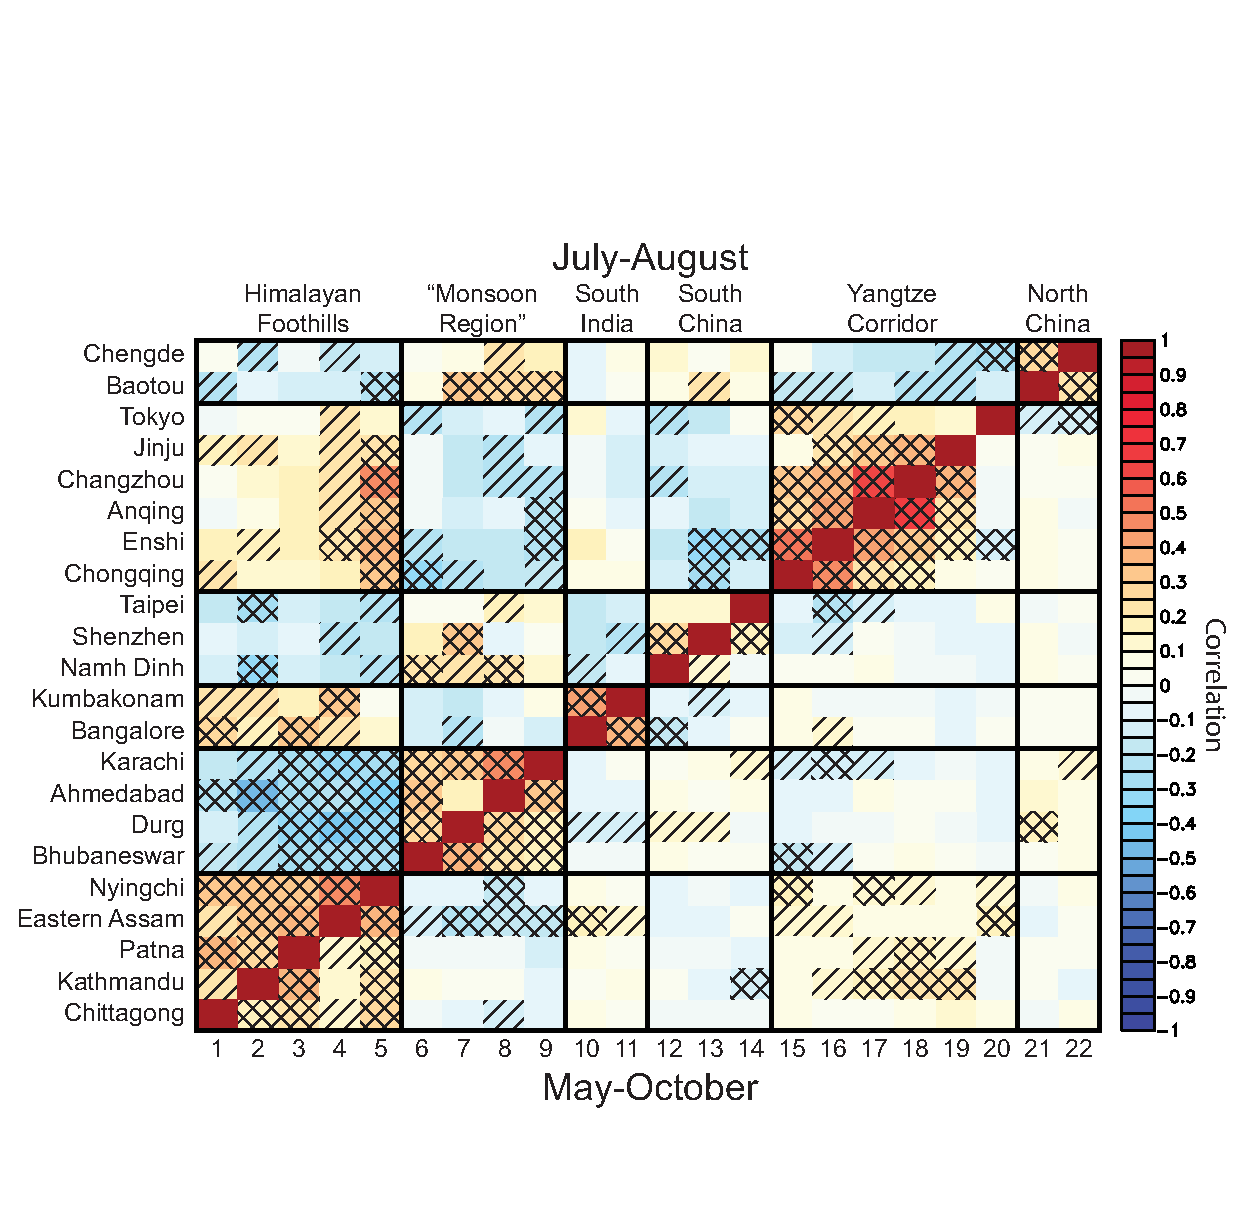
\includegraphics[width=36pc,angle=0]{fig3correl}\\
  \caption{Correlation coefficient $r$ between normalized anomaly precipitation $P''$ at each of the 22 reference points for July-August (JA, upper-left) and May-October (MJJASO, bottom-right). Confidence levels above 95\% and 99\% are indicated by single and double diagonal hashes respectively. July-August - 95\% : $r >.184$, 99\% : $r >.240$; May-October - 95 \% : $r>.106$, 99\% : $r >.139$. Region-to-region correlations reproduce point-to-point results closely (not shown).}\label{f3}
\end{figure}

\begin{figure}[t]
  \noindent\includegraphics[width=36pc,angle=0]{fig4agreement}\\
  \caption{Agreement map $A(x,y)$ of anomalies predicted by all 22 reference points, using method described in text, with 700 meter and 3000 meter topography isolines superimposed.}\label{f4}
\end{figure}

\begin{figure}[t]
  \noindent\includegraphics[width=32pc,angle=0]{fig5eof_allasia}\\
  \caption{Leading July-August spatial and temporal EOFs of normalized anomaly precipitation $P''$ for the region 64E-142E and 5N-45N (All-Asia) with .5\textdegree\ $\times$ .5\textdegree\ resolution and percentage of variance listed alongside. July (white shading) and August (gray shading) value of temporal EOF are shown separately. Time series are normalized to unit variance ($\sigma=1$). Linear best fit lines are superimposed on all time series (dashed line). Trends - EOF 1: .014 yr$^{-1}$ EOF 2: .032 yr$^{-1}$ EOF 3: -.012 yr$^{-1}$ EOF4: -.019 yr$^{-1}$. The trend in EOF 2 surpasses a confidence level of 95\% according to a permutation test, but no other trend is statistically significant.}\label{f5}
\end{figure}

\begin{figure}[t]
  \noindent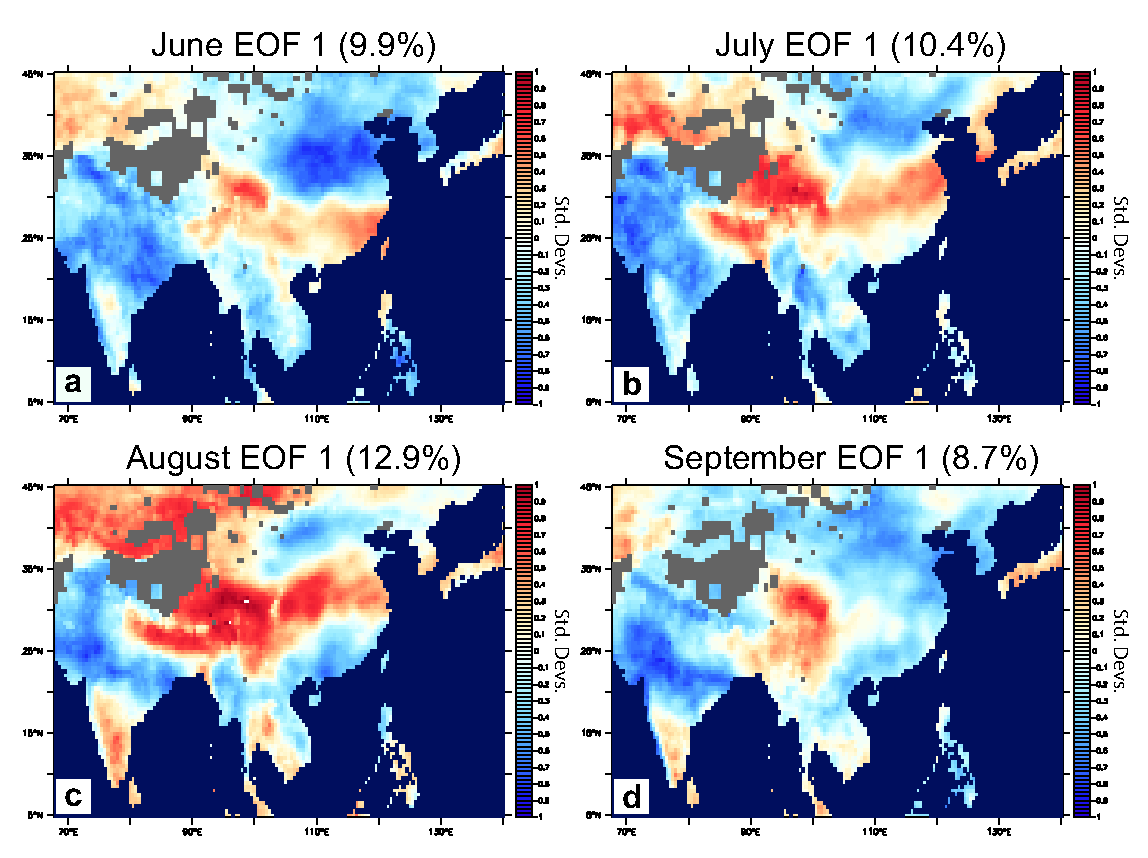
\includegraphics[width=36pc,angle=0]{fig6eof_monthly}\\
  \caption{EOF 1 of normalized anomaly precipitation computed separately for June, July, August and September (units of standard deviation) for the region 68E-140E and 5-45N with .5\textdegree\ $\times$ .5\textdegree\ resolution and percentage of variance listed alongside.}\label{f6}
\end{figure}

\begin{figure}[t]
  \noindent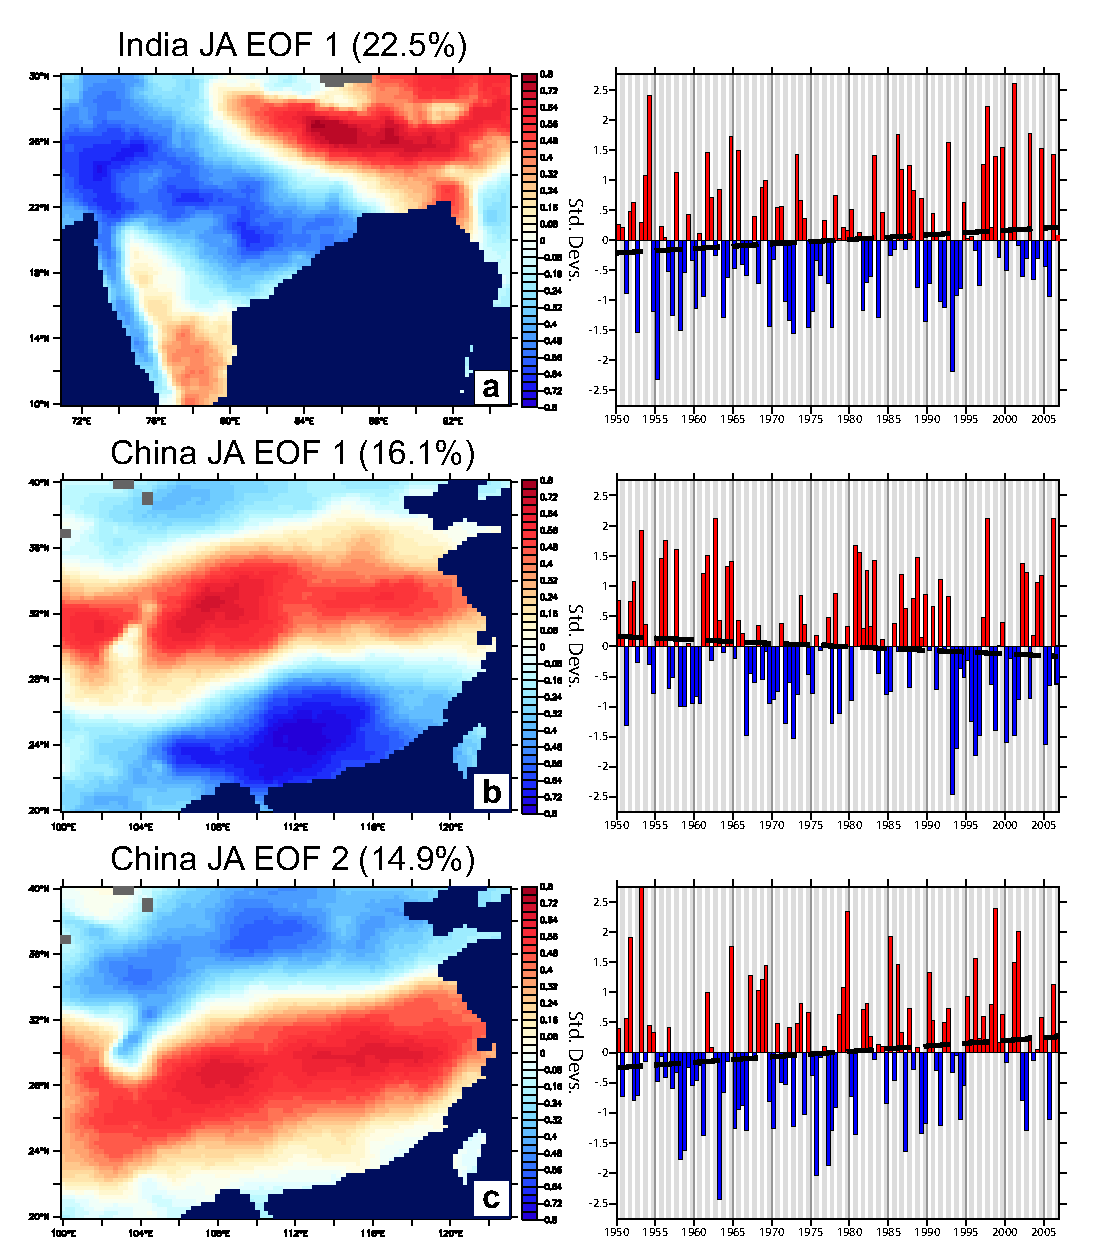
\includegraphics[width=30pc,angle=0]{fig7eof_region}\\
  \caption{Leading EOFs of July-August normalized anomaly precipitation for India (71E-95E and 10N-30N) and China (100E-123E and 20N-40N) with .25\textdegree\ $\times$ .25
  textdegree\ resolution and percentage of variance listed alongside. July (white shading) and August (gray shading) are both shown. Time series are normalized to unit variance ($\sigma=1$). Linear best fit lines are superimposed on all time series (dashed line). Trends - India EOF 1: .019 yr$^{-1}$ China EOF 1: .014 yr$^{-1}$ EOF 2: .022 yr$^{-1}$. No trend is statistically significant at a 95\% level.}\label{f7}
\end{figure}

\begin{figure}[t]
  \noindent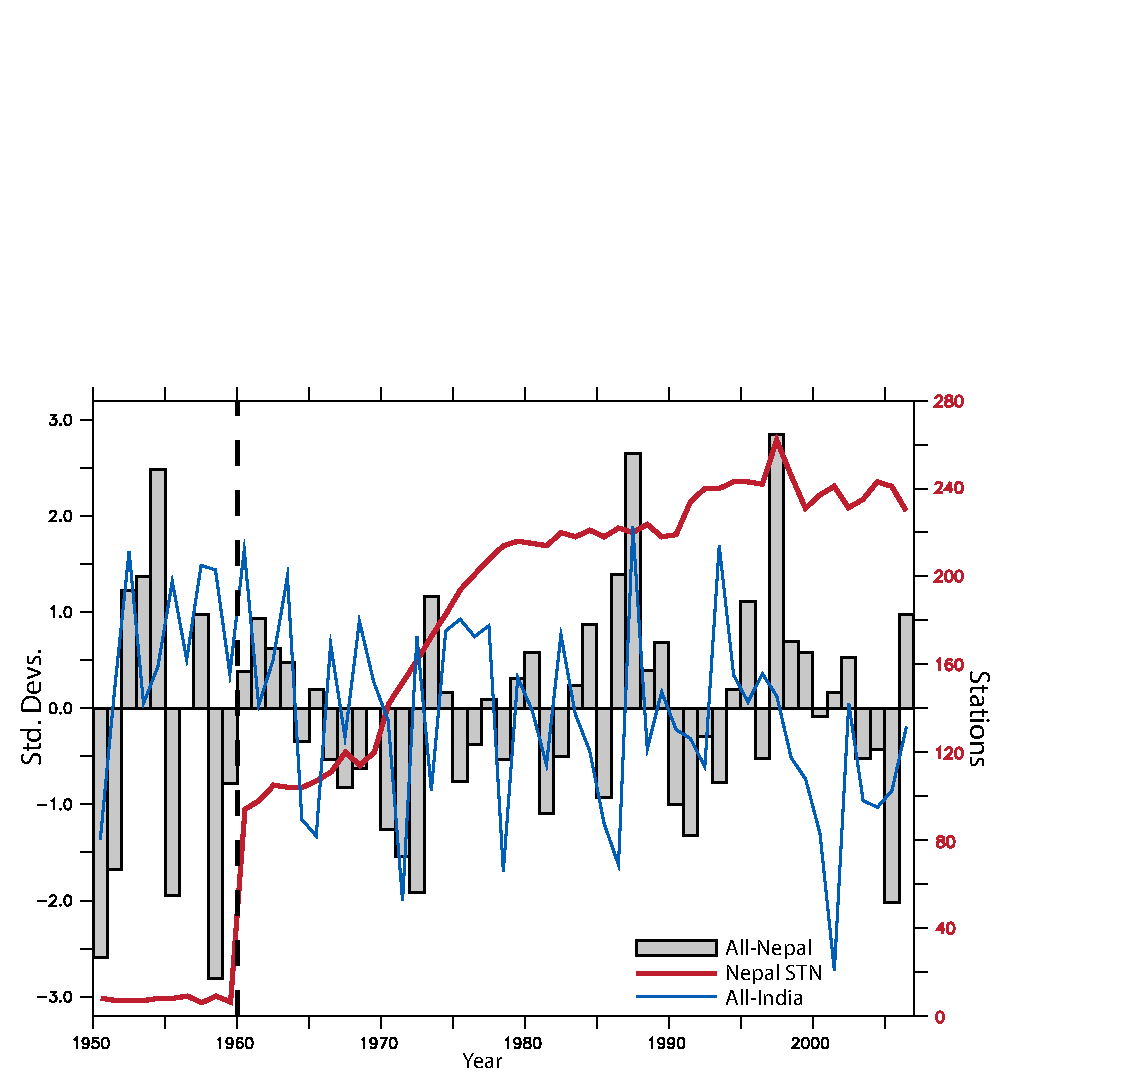
\includegraphics[width=36pc,angle=0]{fig8allnepal}\\
  \caption{Index of July-August All-Nepal monsoon rainfall (gray bars, normalized such that $\sigma= 1$ for 1961-2007) with total number of Nepal stations (red line) and normalized All-India monsoon rainfall (dashed blue line) superimposed. One value is listed per year, obtained by first summing July and August precipitation. Black dotted line marks 1960, after which station coverage in Nepal improves sharply and the use of the All-Nepal index is recommended.}\label{f8}
\end{figure}

\begin{figure}[t]
  \noindent\includegraphics[width=42pc,angle=0]{fig9laglead}\\
  \caption{July-August $K_i^\lambda$ (57-year mean of $C_i^\lambda$) given a reference point $(x_i,y_i)$, defined as anomalous correlation of precipitation anomalies relative to background field with a lag or lead of $\lambda$ days. Variance circles are drawn to include at least 50\% of yearly $C_i^\lambda$ out of all 57 years for each reference point and $\lambda$.}\label{f9}
\end{figure}

\begin{figure}[t]
  \noindent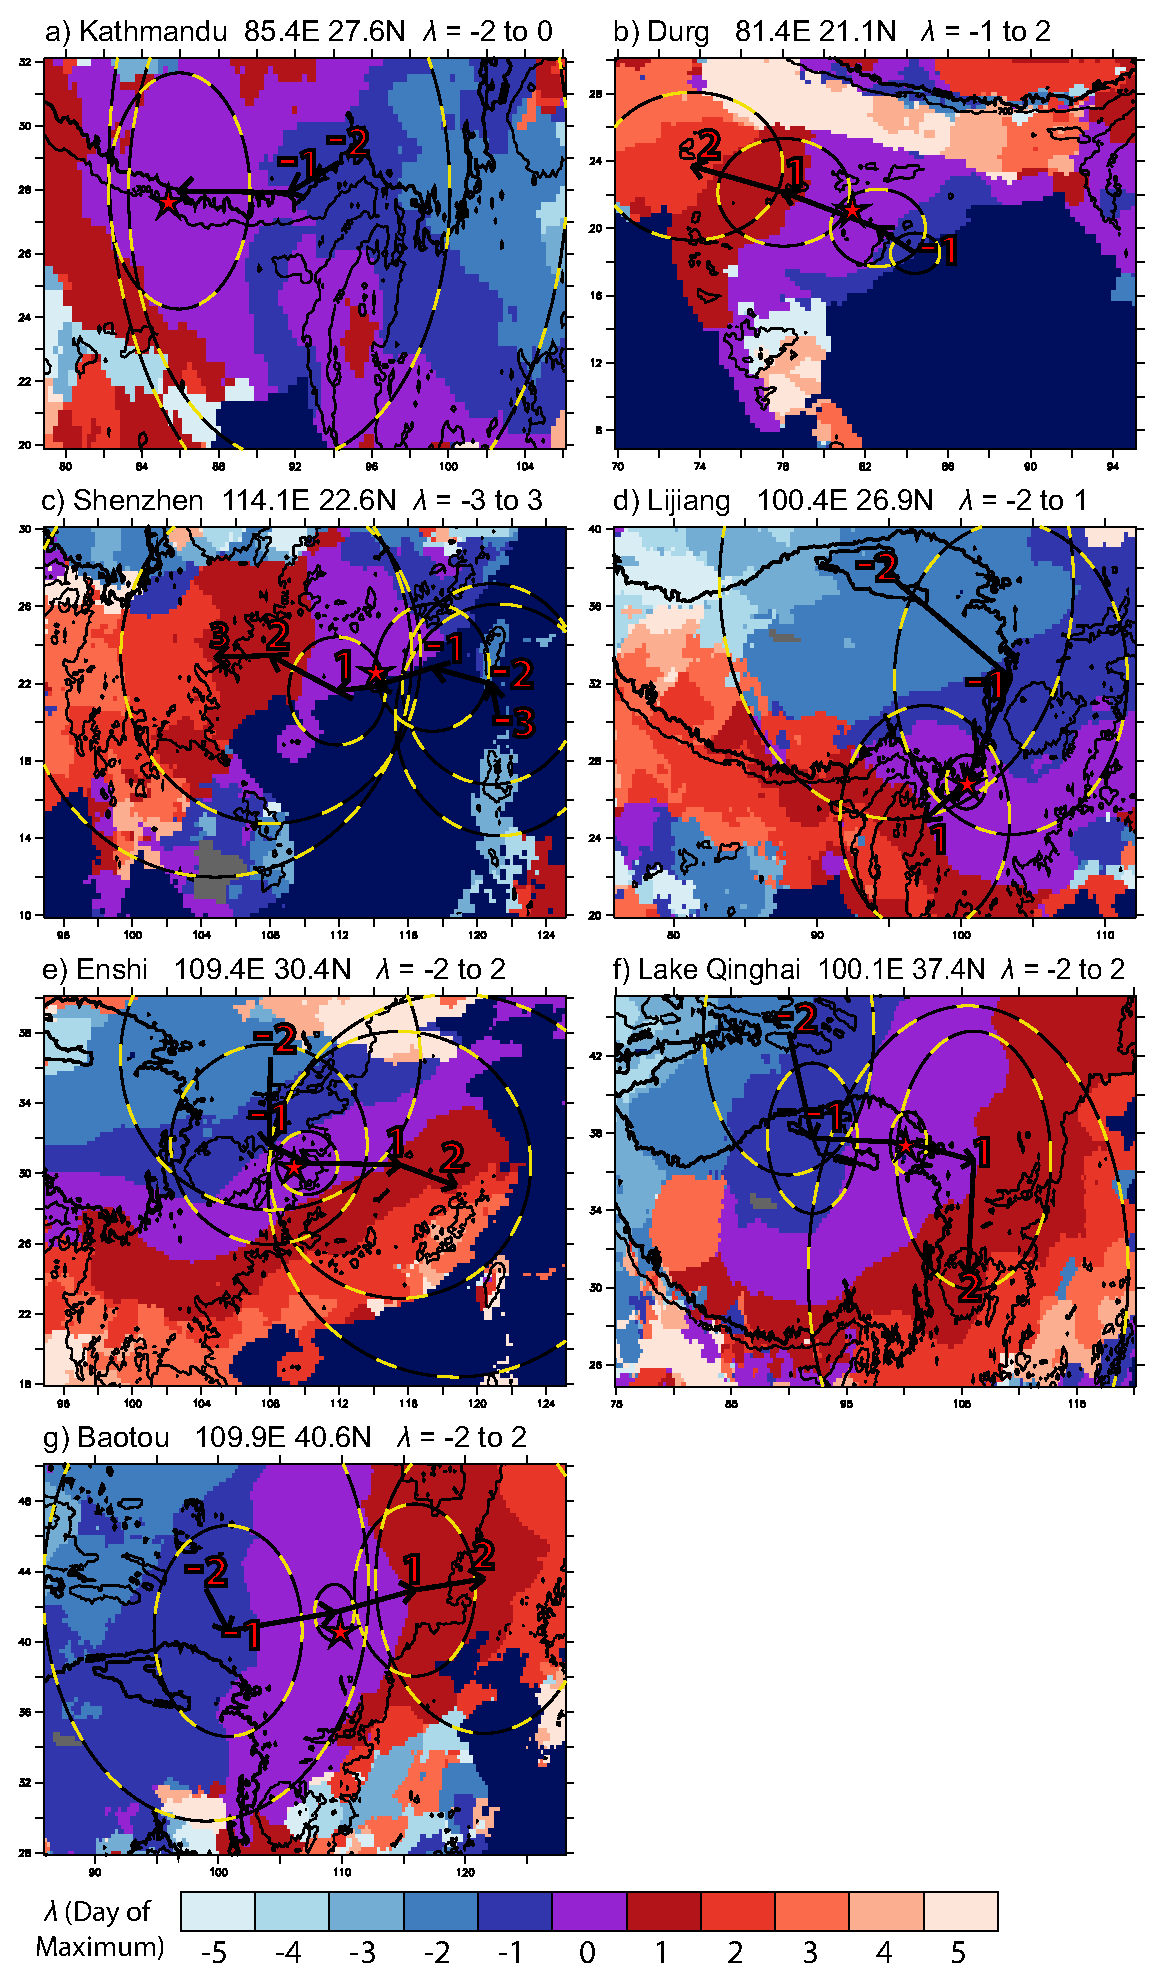
\includegraphics[width=32pc,angle=0]{fig10kmax}\\
  \caption{July-August plot of the day $\lambda$ for which $C_i^\lambda(x,y)$ is maximized at each point. Variance circles from Figure 9 are superimposed for the selection of $\lambda$ listed above each figure.}\label{f10}
\end{figure}

\begin{figure}[t]
  \noindent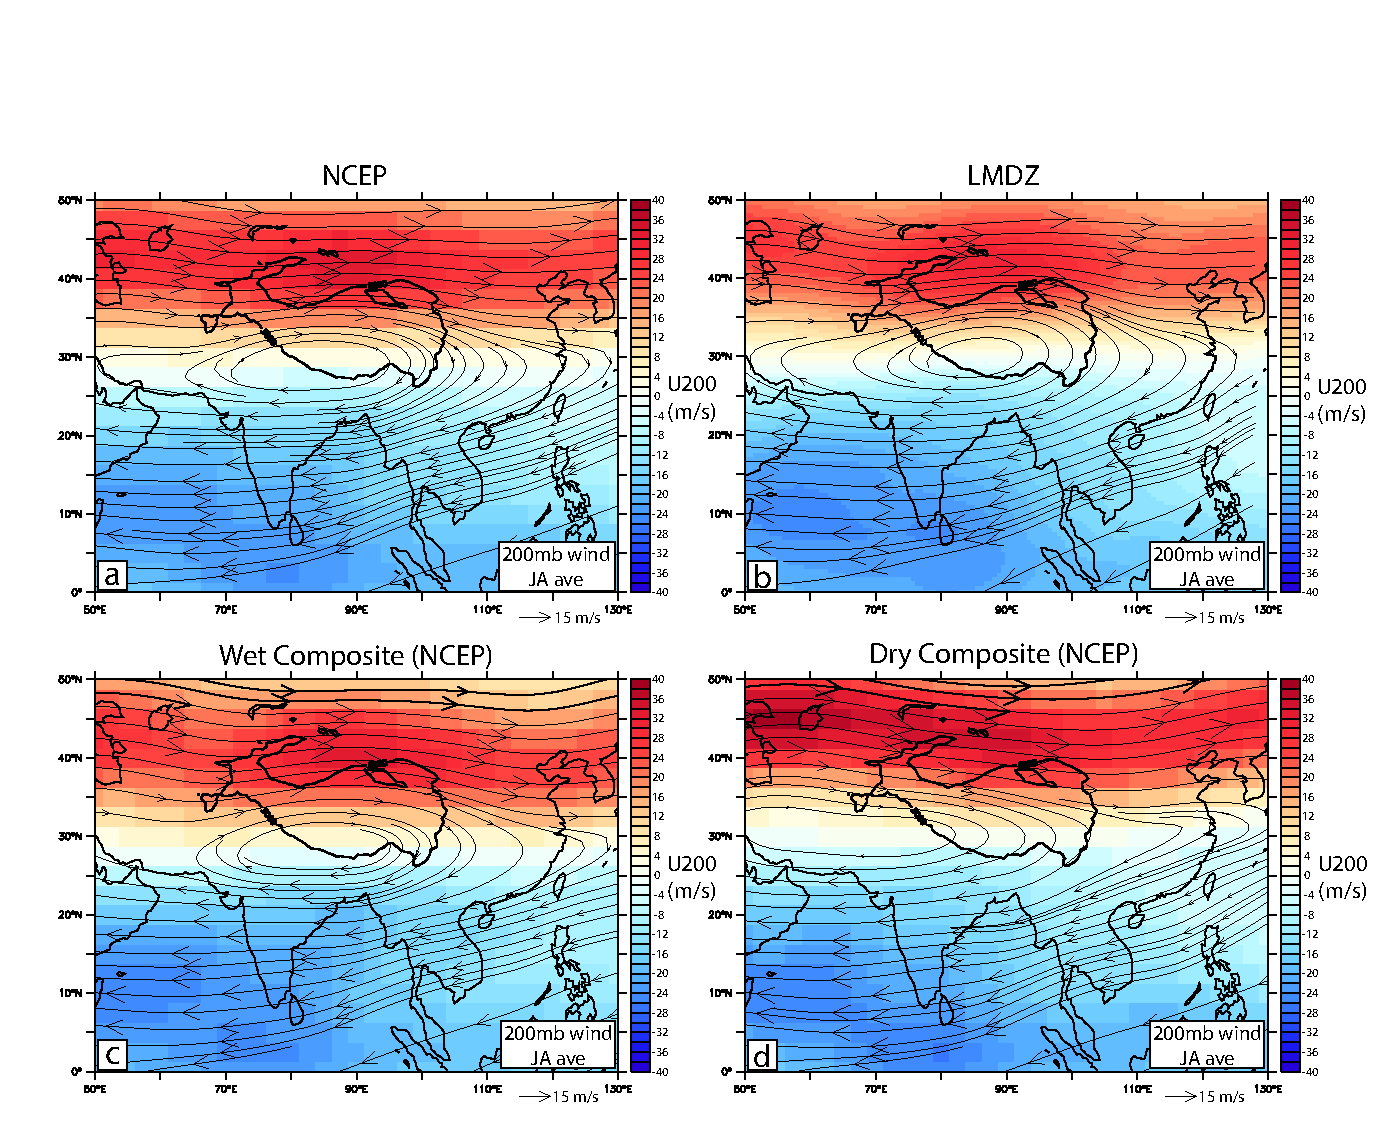
\includegraphics[width=36pc,angle=0]{fig11u200}\\
  \caption{July-August streamlines of mean 200 mb-level winds from NCEP reanalysis (a) and LMDZ (b). Figures c and d are NCEP reanalysis 200 mb-level wind for composites of ``wet'' years (c) and ``dry'' years (d). The ``wet'' composite includes the five years with the most positive value of All-Asia EOF1, while the ``dry'' composite is the equivalent with the five most negative years.}\label{f11}
\end{figure}

\begin{figure}[t]
  \noindent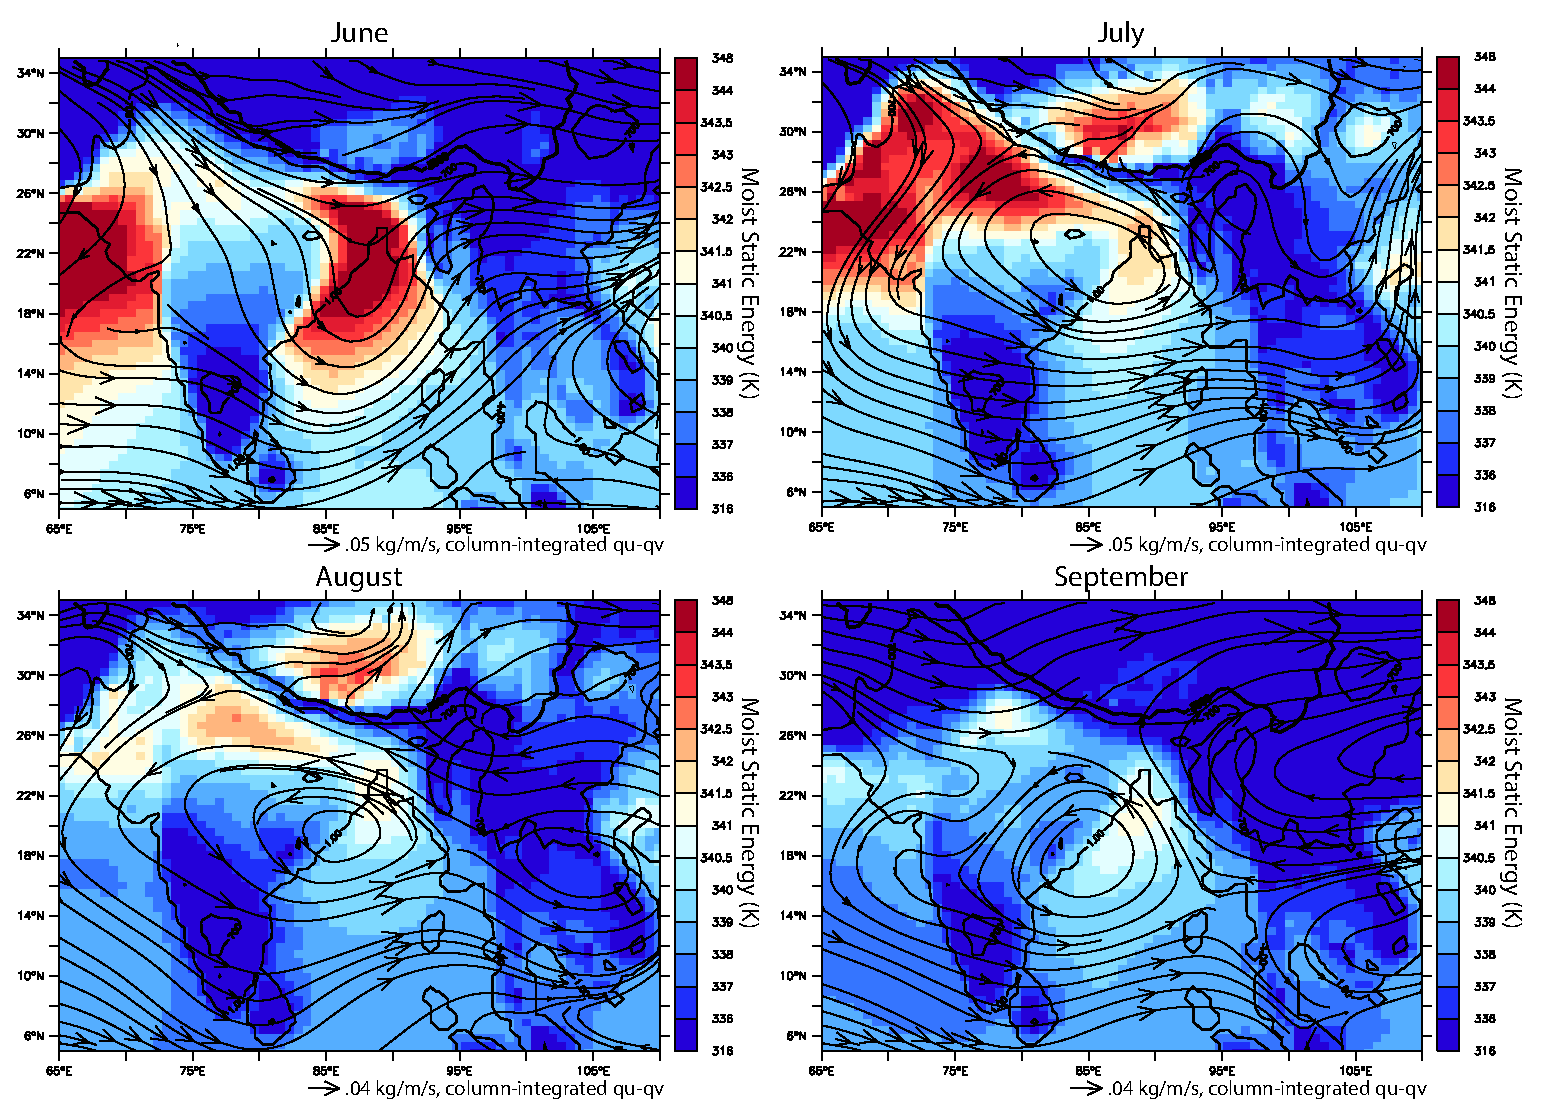
\includegraphics[width=36pc,angle=0]{fig12lmdz}\\
  \caption{Near-surface moist static energy $h_b$ (shading) and column-integrated moisture transport $\overline{q}\overline{u}$\textendash $\overline{qv}$ (vectors) from June to September in LMDZ for the region 65E-110E and 5N-35N. Moist static energy is given by the formula $h_b=c_pT+L_vq+gz$, with specific heat of dry air $c_p$ and latent heat of condensation of water $L_v$ given in main text. Units of moist static energy are Kelvin, obtained by dividing $h_b$ by $c_p$ as practiced in \cite{Boos2013a}. Column-integrated moisture vapor is given by $\overline{qu}=\frac{1}{g}\int q\vec{u}\ \mathrm{d}p $. Note unusual y-axis used to emphasize changes over continental India.}\label{f12}
\end{figure}

%%%%%%%%%%%%%%%%%%%%%%%%%%%%%%%%%%%%%%%%%%%%%%%%%%%%%%%%%%%%%%%%%%%%%
% TABLES
%%%%%%%%%%%%%%%%%%%%%%%%%%%%%%%%%%%%%%%%%%%%%%%%%%%%%%%%%%%%%%%%%%%%%
\begin{table}[t]

\caption{The 22 reference points used in the point to point comparisons and agreement map.}\label{t1}
\begin{center}
\begin{tabularx}{1\textwidth}{ >{\setlength\hsize{2.35\hsize}\centering}X >{\setlength\hsize{.15\hsize}\centering}X >{\setlength\hsize{1.85\hsize}\centering}X >{\setlength\hsize{.8\hsize}\centering}X >{\setlength\hsize{.8\hsize}\centering}X >{\setlength\hsize{1.1\hsize}\centering}X >{\setlength\hsize{.4\hsize}\centering}X >{\setlength\hsize{.4\hsize}\centering}X }
Region & \# & Nearest City & Long & Lat & JA Precip (mm day$^{-1}$) & St. Dev. & STN \tabularnewline
\hline
\multirow{5}{*}{\parbox[t]{3.6cm}{Himalayan Foothills\\ + Bangladesh}} & 1 & Chittagong & 91.9\textdegree E & 22.4\textdegree N & 16.55 & 6.58 & .88 \tabularnewline
& 2 & Kathmandu & 85.4\textdegree E & 27.6\textdegree N & 12.34 & 3.33 & 5.09 \tabularnewline
& 3 & Patna & 85.1\textdegree E & 25.6\textdegree N & 7.78 & 2.92 & 2.42 \tabularnewline
& 4 & Eastern Assam & 95.1\textdegree E & 27.4\textdegree N & 12.62 & 3.27 & 1.04 \tabularnewline
& 5 & Nyingchi & 94.4\textdegree E & 29.6\textdegree N & 3.71 & 1.47 & 1.28 \tabularnewline
\hline
\multirow{4}{*}{``Monsoon Zone''} & 6 & Bhubaneswar & 85.9\textdegree E & 20.4\textdegree N & 10.06 & 3.04 & 1.98 \tabularnewline
& 7 & Durg & 81.4\textdegree E & 21.1\textdegree N & 9.26 & 2.98 & 1.83 \tabularnewline
& 8 & Ahmedabad & 72.6\textdegree E & 23.1\textdegree N & 7.11 & 3.85 & 1.74 \tabularnewline
& 9 & Karachi & 67.1\textdegree E & 24.9\textdegree N & 1.68 & 2.01 & .86 \tabularnewline
\hline
\multirow{2}{*}{South India} & 10 & Bangalore & 77.6\textdegree E & 12.9\textdegree N & 3.04 & 1.78 & 1.89 \tabularnewline
& 11 & Kumbakonam & 79.4\textdegree E & 10.9\textdegree N & 2.29 & 1.62 & 2.94 \tabularnewline
\hline
\multirow{3}{*}{\parbox[t]{3.6cm}{South China}} & 12 & Namh Dinh & 106.1\textdegree E & 20.4\textdegree N & 7.64 & 3.80 & 1.56 \tabularnewline
& 13 & Shenzhen & 114.1\textdegree E & 22.6\textdegree N & 9.78 & 4.41 & 1.01 \tabularnewline
& 14 & Taipei & 121.6\textdegree E & 25.1\textdegree N & 6.59 & 4.62 & 3.36 \tabularnewline
\hline
\multirow{6}{*}{\parbox[t]{3.6cm}{Yangtze Corridor\\+ Korea + Japan}} & 15 & Chongqing & 106.4\textdegree E & 29.6\textdegree N & 4.41 & 2.15 & 1.49 \tabularnewline
& 16 & Enshi & 109.4\textdegree E & 30.4\textdegree N & 5.80 & 3.09 & 1.32 \tabularnewline
& 17 & Anqing & 117.1\textdegree E & 30.6\textdegree N & 4.58 & 3.03 & 1.42 \tabularnewline
& 18 & Changzhou & 119.9\textdegree E & 31.9\textdegree N & 4.39 & 2.37 & 1.14 \tabularnewline
& 19 & Jinju (Korea) & 128.1\textdegree E & 35.1\textdegree N & 7.66 & 4.10 & 1.67 \tabularnewline
& 20 & Tokyo & 139.4\textdegree E & 35.9\textdegree N & 5.35 & 2.86 & 3.33 \tabularnewline
\hline
\multirow{2}{*}{North China} & 21 & Baotou & 109.9\textdegree E & 40.6\textdegree N & 2.47 & 1.26 & 1.08 \tabularnewline
& 22 & Chengde & 117.9\textdegree E & 40.9\textdegree N & 4.50 & 1.99 & 1.98 \tabularnewline

\end{tabularx}

\end{center}

\end{table}

\begin{table}[t]

\caption{Yearly time series of All-Nepal Monsoon Rainfall, calculated as an area average over Nepal. Station quality improves dramatically starting in 1961 such that use of the 1951-1960 component is discouraged. 1961-2007 values are used to calculate monthly average and standard deviation. July-August total mean rainfall over this period is 10.63 mm day$^{-1}$ for the regional average with a standard deviation of 1.07 mm day$^{-1}$. The inaccuracy of the index from 1951 to 1960 is reflected by the relatively high standard deviation of those points.}\label{t2}
\begin{center}
\begin{tabularx}{.9\textwidth}{ >{\setlength\hsize{.1\hsize}\centering}X >{\setlength\hsize{.1\hsize}\centering}X >{\setlength\hsize{.1\hsize}\centering}X  >{\setlength\hsize{.1\hsize}\centering}X >{\setlength\hsize{.1\hsize}\centering}X >{\setlength\hsize{.1\hsize}\centering}X >{\setlength\hsize{.1\hsize}\centering}X >{\setlength\hsize{.1\hsize}\centering}X >{\setlength\hsize{.1\hsize}\centering}X}
Year & Precip & Index & Year & Precip & Index & Year & Precip & Index \tabularnewline
\hline
\textit{1951} & \textit{7.87} & \textit{-2.59} & 1970 & 10.63 & 0.00 & 1989 & 11.05 & 0.39 \tabularnewline
\textit{1952} & \textit{8.84} & \textit{-1.68} & 1971 & 9.29 & -1.26 & 1990 & 11.35 & 0.68 \tabularnewline
\textit{1953} & \textit{11.94} & \textit{1.23} & 1972 & 8.99 & -1.54 & 1991 & 9.56 & -1.00 \tabularnewline
\textit{1954} & \textit{12.09} & \textit{1.37} & 1973 & 8.57 & -1.92 & 1992 & 9.22 & -1.32 \tabularnewline
\textit{1955} & \textit{13.27} & \textit{2.48} & 1974 & 11.86 & 1.16 & 1993 & 10.32 & -0.29 \tabularnewline
\textit{1956} & \textit{8.54} & \textit{-1.95} & 1975 & 10.80 & 0.16 & 1994 & 9.80 & -0.77 \tabularnewline
\textit{1957} & \textit{10.63} & \textit{0.00} & 1976 & 9.81 & -0.76 & 1995 & 10.83 & 0.19 \tabularnewline
\textit{1958} & \textit{11.68} & \textit{0.98} & 1977 & 10.23 & -0.38 & 1996 & 11.82 & 1.11 \tabularnewline
\textit{1959} & \textit{7.63} & \textit{-2.81} & 1978 & 10.73 & 0.09 & 1997 & 10.07 & -0.52 \tabularnewline
\textit{1960} & \textit{9.80} & \textit{-0.78} & 1979 & 10.06 & -0.53 & 1998 & 13.67 & 2.85 \tabularnewline
1961 & 11.03 & 0.38  & 1980 & 10.96 & 0.31 & 1999 & 11.36 & 0.69 \tabularnewline
1962 & 11.62 & 0.93  & 1981 & 11.25 & 0.58 & 2000 & 11.25 & 0.58 \tabularnewline
1963 & 11.29 & 0.62  & 1982 & 9.46 & -1.09 & 2001 & 10.53 & -0.09 \tabularnewline
1964 & 11.14 & 0.48  & 1983 & 10.09 & -0.50 & 2002 & 10.80 & 0.16 \tabularnewline
1965 & 10.25 & -0.35  & 1984 & 10.89 & 0.24 & 2003 & 11.19 & 0.53 \tabularnewline
1966 & 10.83 & 0.19  & 1985 & 11.55 & 0.87 & 2004 & 10.07 & -0.52 \tabularnewline
1967 & 10.06 & -0.53  & 1986 & 9.63 & -0.93 & 2005 & 10.16 & -0.43 \tabularnewline
1968 & 9.75 & -0.82  & 1987 & 12.11 & 1.39 & 2006 & 8.47 & -2.02 \tabularnewline
1969 & 9.96 & -0.63  & 1988 & 13.45 & 2.65 & 2007 & 11.68 & 0.98 \tabularnewline

\end{tabularx}
\end{center}

\end{table}

\begin{table}[t]

\caption{July-August correlation coefficients $r$ from 1951 to 2007 of All-Nepal rainfall, All-India rainfall (calculated from APHRODITE),``Monsoon Zone'' rainfall and Yangtze rainfall (mean rainfall over the region bounded by (104.5\textdegree E 29\textdegree N), (108\textdegree E 32\textdegree N), (120\textdegree E 34\textdegree N) and (122\textdegree E 31.5\textdegree N)), as well as Oceanic Ni\~no Index (ONI) in preceding December, or equivalently the N(0)-D(0)-J(1) mean of Ni\~no 3.4 (SST anomaly averaged over the region 5\textdegree S-5\textdegree N and 120\textdegree W-170\textdegree W). Each time series is compared with All-Asia temporal EOF 1, India temporal EOF 1, China temporal EOFs 1 \& 2 and official All-India Monsoon Rainfall from the Indian Meteorological Department (IMD). Although All-Nepal Monsoon Rainfall is reliable only for 1961-2007 due to station coverage limitations and the Monsoon Zone time series likewise degrades after 1970, all 57 years are used for consistency, and results are not substantially affected. July and August are treated as separate time points except for correlation with ONI, which uses yearly values. 95\% and 99\% confidence levels are indicated by bold font and asterisks respectively.}\label{t3}
\begin{center}
\begin{tabularx}{1\textwidth}{>{\setlength\hsize{.16\hsize}\centering\arraybackslash}X >{\setlength\hsize{.09\hsize}\centering\arraybackslash}X >{\setlength\hsize{.09\hsize}\centering\arraybackslash}X >{\setlength\hsize{.08\hsize}\centering\arraybackslash}X >{\setlength\hsize{.07\hsize}\centering\arraybackslash}X >{\setlength\hsize{.14\hsize}\centering\arraybackslash}X >{\setlength\hsize{.10\hsize}\centering\arraybackslash}X >{\setlength\hsize{.17\hsize}\centering\arraybackslash}X  >{\setlength\hsize{.10\hsize}\centering\arraybackslash}X}
Index & All-Nepal & All-India & MZ & YZ & EOF 1 (All-Asia) & EOF 1 (India) & EOF 1/2 (China) & All-India (IMD) \tabularnewline
\hline
All-Nepal & \textbf{1*} & -.07 & \textbf{-.31*} & \textbf{.28*} & \textbf{.59*} &  \textbf{.70*} &  \textbf{.34*}/.10 & .02 \tabularnewline
All-India & -.07 & \textbf{1*} & \textbf{.82*} & -.08 & \textbf{-.44*} &  \textbf{-.54*} &  -.04/ \textbf{-.28*} &  \textbf{.95*} \tabularnewline
Monsoon Zone &  \textbf{-.31*} &  \textbf{.82*} & \textbf{1*} & \textbf{-.24} &\textbf{-.77*} &  \textbf{-.88*} & \textbf{.30*}/\textbf{-.46*} &  \textbf{.78*} \tabularnewline
Yangtze & \textbf{.28*} & -.08 & \textbf{-.24} & \textbf{1*} & \textbf{.62*} & \textbf{.32*} & \textbf{.62*}/\textbf{.62*} & -.11 \tabularnewline
Oceanic Ni\~no Index & .11 & .26 & .17 & .15 & .11 & -.02 & .17/-.11 & .25 \tabularnewline
\end{tabularx}
\end{center}

\end{table}

\end{document}